% =============================================================================
% Plantilla de paper — Laboratorio 4: Capa de Red (OMNeT++)
% Cátedra de Redes y Sistemas Distribuidos — FaMAF/UNC
%
% Compilación:
%   pdflatex lab4-paper.tex
%   pdflatex lab4-paper.tex
%
% Carpeta figuras/: coloque ahí PDF/PNG exportados desde OMNeT++ o scripts.
% =============================================================================

\documentclass[10pt,letterpaper,twocolumn]{article}

\usepackage[T1]{fontenc}
\usepackage[utf8]{inputenc}
\usepackage[english]{babel}
\usepackage[margin=0.9in]{geometry}
\usepackage{amsmath,amsfonts}
\usepackage{graphicx}
\usepackage{booktabs}
\usepackage{multirow}
\usepackage{subcaption}
\usepackage{xcolor}
\usepackage{url}
\usepackage[hidelinks]{hyperref}
\usepackage{tikz}
\usepackage{pgfplots}
\pgfplotsset{compat=1.18}
\usetikzlibrary{arrows.meta}
\usepackage{placeins}

% Tablas que deben caber dentro de una columna (formato 2 columnas)
\newcommand{\coltablesetup}{%
  \scriptsize
  \setlength{\tabcolsep}{3pt}%
  \renewcommand{\arraystretch}{1.08}%
}

% Datos del grupo — modifique estos campos
\newcommand{\Titulo}{Routing Strategies for Ring and General Topologies in OMNeT++}
\newcommand{\Grupo}{Grupo 25}
\newcommand{\Integrantes}{Gerbaudo, Nicolás Ignacio; Jorge González, Nicolás; Ontivero, Nahuel Mauricio; Vides, Alejo Miguel}
\renewcommand{\refname}{Referencias}
\renewcommand{\abstractname}{Abstract}
\renewcommand{\appendixname}{Ap\'{e}ndice}

% Entorno estilo revista para metadatos en inglés
\newenvironment{IEEEkeywords}{%
  \smallskip\noindent\textbf{Index Terms---}%
}{\par\smallskip}

\begin{document}

\twocolumn[
\begin{@twocolumnfalse}
  \begin{center}
    {\LARGE\bfseries \Titulo\par}
    \vspace{0.6em}
    {\normalsize \Integrantes\par}
    \vspace{0.4em}
    {\small \Grupo, Facultad de Matemática, Astronomía, Física y Computación (FaMAF)\\
    Universidad Nacional de Córdoba, Argentina\par}
    \vspace{1em}
  \end{center}

  \begin{abstract}
  \noindent
  This paper analyzes and compares two routing strategies for a simulated ring network of 8 nodes implemented in OMNeT++. The baseline algorithm, provided as a kickstarter, always forwards packets through \texttt{lnk[0]}, concentrating all traffic in one direction of the ring and leaving half the network capacity unused. We instrumented the model with five metrics: end-to-end delay, hop count, buffer occupancy, link utilization, and forwarded packets per node. Two traffic scenarios were evaluated: Scenario 1, where only two nodes transmit to a single destination, and Scenario 2, where seven nodes simultaneously transmit to the same destination with varying inter-arrival times. Results show that the baseline saturates quickly, reaching average delays of over 50 seconds in Scenario 1 and requiring an inter-arrival time of at least 7 seconds to achieve stability in Scenario 2. The proposed algorithm selects the shortest path in both ring directions and uses buffer occupancy as a tiebreaker, reducing average delay by 86.5\% in Scenario 1 and significantly improving performance in Scenario 2 under moderate and low load conditions. No routing loops were observed, as the algorithm always advances packets toward the destination. Both algorithms remain vulnerable to node failures due to the absence of dynamic topology discovery mechanisms.
  \end{abstract}

  \begin{IEEEkeywords}
  Network simulation, OMNeT++, routing, ring topology, performance evaluation,
  queueing, stability.
  \end{IEEEkeywords}

  \vspace{0.5em}
\end{@twocolumnfalse}
]

\selectlanguage{english}
% Contenido principal en español (sin babel-spanish; títulos de sección en español manualmente)

\section{Introducción}
\label{sec:intro}

Este artículo aborda el problema del enrutamiento en una red en anillo de 8 nodos simulada en OMNeT++. Cada nodo cuenta con una capa de aplicación (\texttt{app}), una capa de red (\texttt{net}) y dos capas de enlace (\texttt{lnk[0]} y \texttt{lnk[1]}), que conectan al nodo con sus dos vecinos. El objetivo es analizar el comportamiento del algoritmo de enrutamiento provisto por la cátedra, identificar sus limitaciones y evaluar el rendimiento del sistema bajo distintos escenarios de tráfico. El resto del artículo se organiza de la siguiente manera: la Sección~\ref{sec:modelo} describe el escenario y las métricas, la Sección~\ref{sec:analisis} analiza el baseline, la Sección~\ref{sec:diseno} presenta el algoritmo propuesto, la Sección~\ref{sec:evaluacion} compara ambos enfoques y la Sección~\ref{sec:conclusiones} resume las conclusiones.

En el algoritmo del kickstarter, cada nodo evalúa si es el destino final del paquete recibido: de serlo, lo entrega a su capa de aplicación; de lo contrario, lo reenvía siempre por la interfaz \texttt{toLnk[0]}, sin considerar la distancia ni el estado de la red, lo que implica que el tráfico siempre se envía en sentido horario a lo largo del anillo hasta llegar al destino. En consecuencia, la mitad de la capacidad de la red queda sin utilizar y ciertos enlaces concentran todo el tráfico, mientras otros permanecen inactivos; así se genera saturación en los buffers y demoras crecientes. Consideramos que una estrategia es mejor cuando reduce la demora media, disminuye la ocupación de buffers y aprovecha ambos sentidos del anillo sin generar bucles de enrutamiento. En este trabajo evaluamos el rendimiento del sistema mediante métricas de demora extremo a extremo, ocupación de buffers, utilización de enlaces, cantidad de saltos por paquete y paquetes en tránsito por nodo.

El algoritmo propuesto elige la ruta más corta en ambas direcciones del anillo y, en caso de empate, desempata por congestión consultando la ocupación de los buffers locales. Los resultados muestran mejoras significativas en demora y cantidad de saltos en la mayoría de los escenarios evaluados.

\section{Escenario y modelo de simulación}
\label{sec:modelo}

\subsection{Topología y configuración de tráfico}

La red simulada consiste en un anillo de 8 nodos (\texttt{node[0]} a \texttt{node[7]}), donde cada nodo se conecta con sus dos vecinos mediante enlaces \textit{full-duplex} de 1\,Mbps y 100\,µs de retardo. Cada nodo cuenta con tres capas:
\begin{itemize}
  \item una capa de aplicación (\texttt{app}), que genera y recibe paquetes;
  \item una capa de red (\texttt{net}), que decide por qué interfaz reenviar cada paquete; y
  \item dos capas de enlace (\texttt{lnk[0]} y \texttt{lnk[1]}), cada una conectada a uno de los vecinos.
\end{itemize}
La topología de la red y la estructura interna de un nodo se muestran en las Figs.~\ref{fig:topologia-red} y~\ref{fig:topologia-nodo-0}, respectivamente.

\begin{figure}[!t]
  \centering
  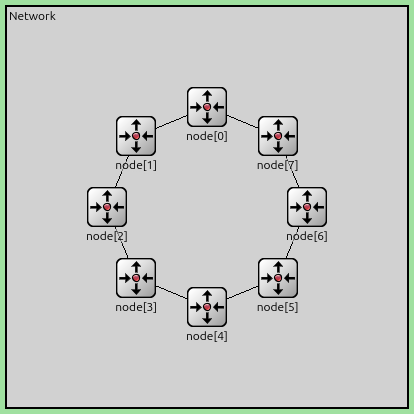
\includegraphics[width=\columnwidth]{../../figuras/topologia-red.png}
  \caption{Topología en anillo de 8 nodos.}
  \label{fig:topologia-red}
\end{figure}

\begin{figure}[!t]
  \centering
  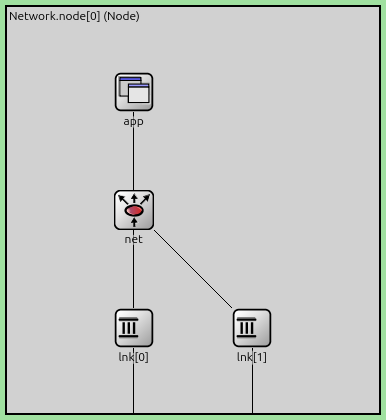
\includegraphics[width=\columnwidth]{../../figuras/topologia-nodo-0.png}
  \caption{Estructura interna de \texttt{node[0]}: \texttt{lnk[0]} conecta con \texttt{node[7]} y \texttt{lnk[1]} conecta con \texttt{node[1]}.}
  \label{fig:topologia-nodo-0}
\end{figure}

\begin{table}[!ht]
  \centering
  \caption{Configuración experimental por escenario.}
  \label{tab:config}
  \coltablesetup
  \resizebox{\columnwidth}{!}{%
  \begin{tabular}{@{}lcc@{}}
    \toprule
    \textbf{Parámetro} & \textbf{Caso 1} & \textbf{Caso 2} \\
    \midrule
    Fuentes activas & \texttt{n[0]}, \texttt{n[2]} & \texttt{n[0--4]}, \texttt{n[6--7]} \\
    Destino & \texttt{n[5]} & \texttt{n[5]} \\
    \texttt{packetByteSize} & 125000 & 125000 \\
    \texttt{interArrivalTime} & \texttt{exp(1)} & \texttt{exp(0.5--10)} \\
    T. simulación (s) & 200 & 200 \\
    Semilla & 0 (default) & 0 (default) \\
    \bottomrule
  \end{tabular}%
  }
\end{table}

\FloatBarrier

\subsection{Métricas registradas}
\label{sec:metricas}

Las métricas se instrumentaron directamente en los módulos del modelo:

\begin{itemize}
  \item \textbf{Demora extremo a extremo:} tiempo transcurrido desde que un paquete se crea en la \texttt{app} origen hasta que se recibe en la \texttt{app} destino. Se calcula como la diferencia entre el tiempo actual y el tiempo de creación del paquete, y se registra en \texttt{app} como vector (una muestra por paquete\footnote{Cada vez que llega un paquete se registra un punto en el vector, es decir, el vector tiene tantos puntos como paquetes recibidos.}) y como escalar (promedio final).
  \item \textbf{Saltos por paquete:} número de saltos que realiza un paquete desde su origen hasta su destino. El campo \texttt{hopCount} se incrementa en \texttt{net} en cada reenvío y se lee en \texttt{app} al recibir el paquete. Se registra como vector y como escalar (promedio final).
  \item \textbf{Ocupación de buffers:} cantidad de paquetes en espera en la cola de cada \texttt{lnk}. Se registra como vector cada vez que el tamaño de la cola cambia.
  \item \textbf{Utilización de enlaces:} fracción del tiempo de simulación durante la cual cada \texttt{lnk} estuvo transmitiendo activamente. Se acumula en \texttt{lnk} sumando el \texttt{serviceTime} de cada paquete transmitido y se reporta como escalar al final dividiendo por el tiempo total de simulación.
  \item \textbf{Paquetes en tránsito por nodo:} cantidad total de paquetes ajenos que cada \texttt{net} reenvió durante la simulación. Se cuenta en \texttt{net} como escalar.
\end{itemize}

\begin{table}[!ht]
  \centering
  \caption{Métricas instrumentadas en el simulador.}
  \label{tab:metricas}
  \coltablesetup
  \resizebox{\columnwidth}{!}{%
  \begin{tabular}{@{}lccc@{}}
    \toprule
    \textbf{Métrica} & \textbf{Módulo} & \textbf{Tipo} & \textbf{Unid.} \\
    \midrule
    Demora E2E            & \texttt{app} & vector + escalar & s \\
    Saltos / paquete      & \texttt{app} & vector + escalar & adim. \\
    Ocupación buffer      & \texttt{lnk} & vector           & pkts \\
    Utilización enlace    & \texttt{lnk} & escalar          & \% \\
    Paquetes en tránsito  & \texttt{net} & escalar          & adim. \\
    \bottomrule
  \end{tabular}%
  }
\end{table}

\FloatBarrier

\section{Tarea de análisis: evaluación del kickstarter}
\label{sec:analisis}

\subsection{Caso 1: tráfico configurado (\texttt{node[0]} y \texttt{node[2]} $\rightarrow$ \texttt{node[5]})}

\textbf{\textit{Configuración experimental.}} Sólo \texttt{node[0]} y \texttt{node[2]} transmiten hacia \texttt{node[5]} con \texttt{interArrivalTime} distribuido exponencialmente con media de 1 segundo y paquetes de 125000 bytes. El resto de los nodos no genera tráfico. La simulación corre durante 200 segundos.

\textbf{\textit{Métricas obtenidas.}} Las métricas registradas durante la simulación se describen en la Sección~\ref{sec:metricas}.

\textbf{\textit{Uso de recursos.}} Los recursos de la red se utilizan de forma muy desigual. Dado que el algoritmo del kickstarter reenvía todos los paquetes por \texttt{lnk[0]} (sentido horario), sólo 5 de las 8 interfaces \texttt{lnk[0]} transportan paquetes, mientras que todas las interfaces \texttt{lnk[1]} permanecen inactivas.

El enlace más cargado es \texttt{node[0].lnk[0]}, con una utilización del 99.5\% y una ocupación media de buffer de 92.92 paquetes (Tabla~\ref{tab:caso1}), lo que indica saturación sostenida. Esto se debe a que por este enlace pasan los paquetes generados por \texttt{node[0]} y \texttt{node[2]}. La Fig.~\ref{fig:entrega-parcial-caso1_buffers_fuentes} confirma que el buffer de \texttt{node[0].lnk[0]} crece de forma sostenida a lo largo de la simulación, mientras que el de \texttt{node[2].lnk[0]} se mantiene relativamente acotado.

Los nodos intermediarios \texttt{node[1]}, \texttt{node[6]} y \texttt{node[7]} muestran una ocupación de buffer máxima de 1 paquete (Fig.~\ref{fig:entrega-parcial-caso1_buffers_intermediarios}), a pesar de utilizar sus enlaces entre el 93.5\% y el 99\%. Esto refleja que los paquetes fluyen de forma casi continua pero sin acumulación significativa en esos nodos.

En cuanto a los paquetes reenviados (Fig.~\ref{fig:entrega-parcial-caso1_forwarded}), \texttt{node[6]} y \texttt{node[7]} reenvían aproximadamente 197 y 198 paquetes respectivamente. Dado que ambas fuentes generan aproximadamente 200 paquetes cada una y ambos nodos están en la ruta de las dos fuentes, se esperaría que reenviaran unos 400 paquetes. El hecho de que sólo hayan reenviado unos 200 es evidencia adicional de saturación: gran parte de los paquetes quedaron atrapados en los buffers al finalizar la simulación.

\begin{table}[!ht]
 \centering
 \caption{Resultados del Caso~1 (baseline kickstarter).}
 \label{tab:caso1}
 \resizebox{\columnwidth}{!}{%
 \begin{tabular}{@{}lrr@{}}
   \toprule
   \textbf{Métrica} & \textbf{Prom.} & \textbf{Desv.} \\
   \midrule
   Demora extremo a extremo (s) & 51.16 & --- \\
   Saltos por paquete           & 3.92  & --- \\
   \midrule
   \multicolumn{3}{@{}l}{\textit{Utilización de enlace (\%)}} \\
   \quad node[0].lnk[0] & 99.5 & --- \\
   \quad node[1].lnk[0] & 93.5 & --- \\
   \quad node[2].lnk[0] & 94.0 & --- \\
   \quad node[6].lnk[0] & 98.5 & --- \\
   \quad node[7].lnk[0] & 99.0 & --- \\
   \midrule
   \multicolumn{3}{@{}l}{\textit{Ocupación de buffer (paquetes)}} \\
   \quad node[0].lnk[0] & 92.92 & 54.83 \\
   \quad node[1].lnk[0] & 0.50  & 0.50  \\
   \quad node[2].lnk[0] & 3.29  & 2.51  \\
   \quad node[6].lnk[0] & 0.50  & 0.50  \\
   \quad node[7].lnk[0] & 0.50  & 0.50  \\
   \midrule
   \multicolumn{3}{@{}l}{\textit{Paquetes reenviados por nodo}} \\
   \quad node[0] & 186 & --- \\
   \quad node[1] & 187 & --- \\
   \quad node[6] & 197 & --- \\
   \quad node[7] & 198 & --- \\
   \bottomrule
 \end{tabular}%
 }
 {\footnotesize
 \begin{flushleft}
 El resto de los enlaces tiene utilización 0\%. \\
 Los \texttt{node[3].lnk[0]}, \texttt{node[4].lnk[0]} y \texttt{node[5].lnk[0]} no registraron ocupación de buffer por no haber tenido tráfico en sus colas durante la simulación. \\
 El resto de los nodos reenvió 0 paquetes.
 \end{flushleft}
 }
\end{table}

\begin{figure}[!ht]
 \centering
 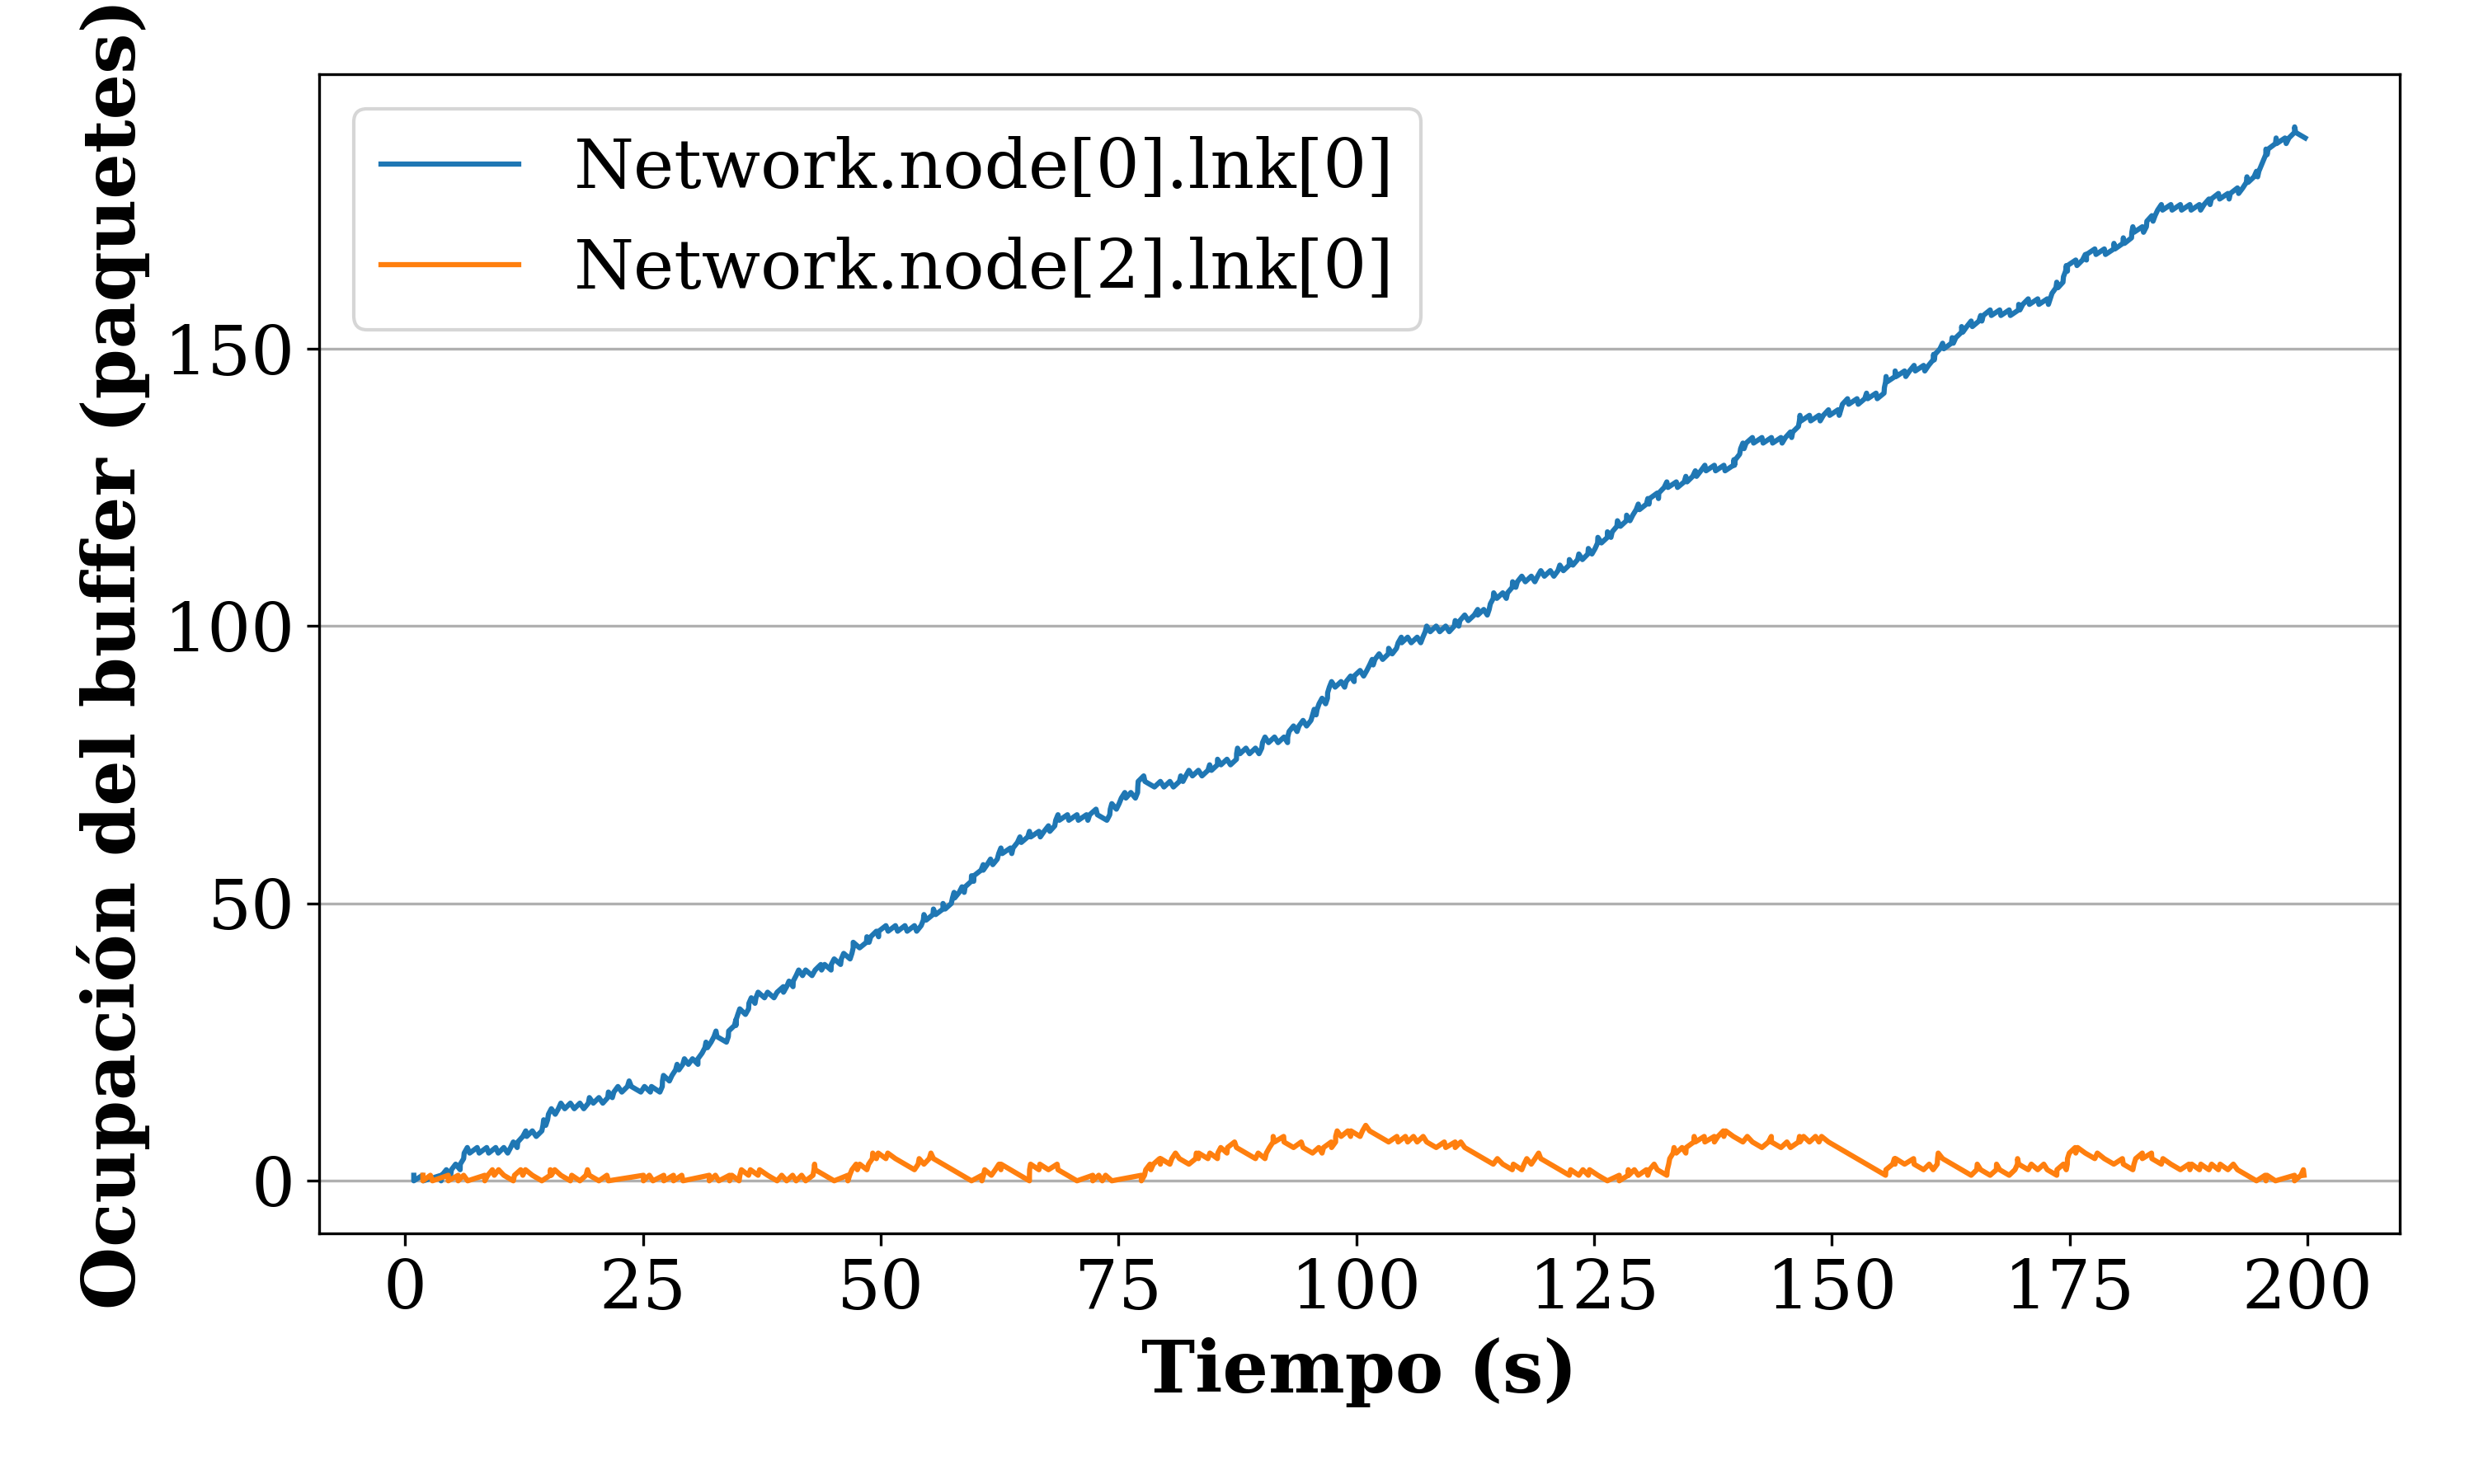
\includegraphics[width=\columnwidth]{../../figuras/entrega-parcial-caso1_buffers_fuentes.png}
 \caption{Ocupación de buffers a lo largo del tiempo --- nodos fuente (node[0] y node[2]).}
 \label{fig:entrega-parcial-caso1_buffers_fuentes}
\end{figure}

\begin{figure}[!ht]
 \centering
 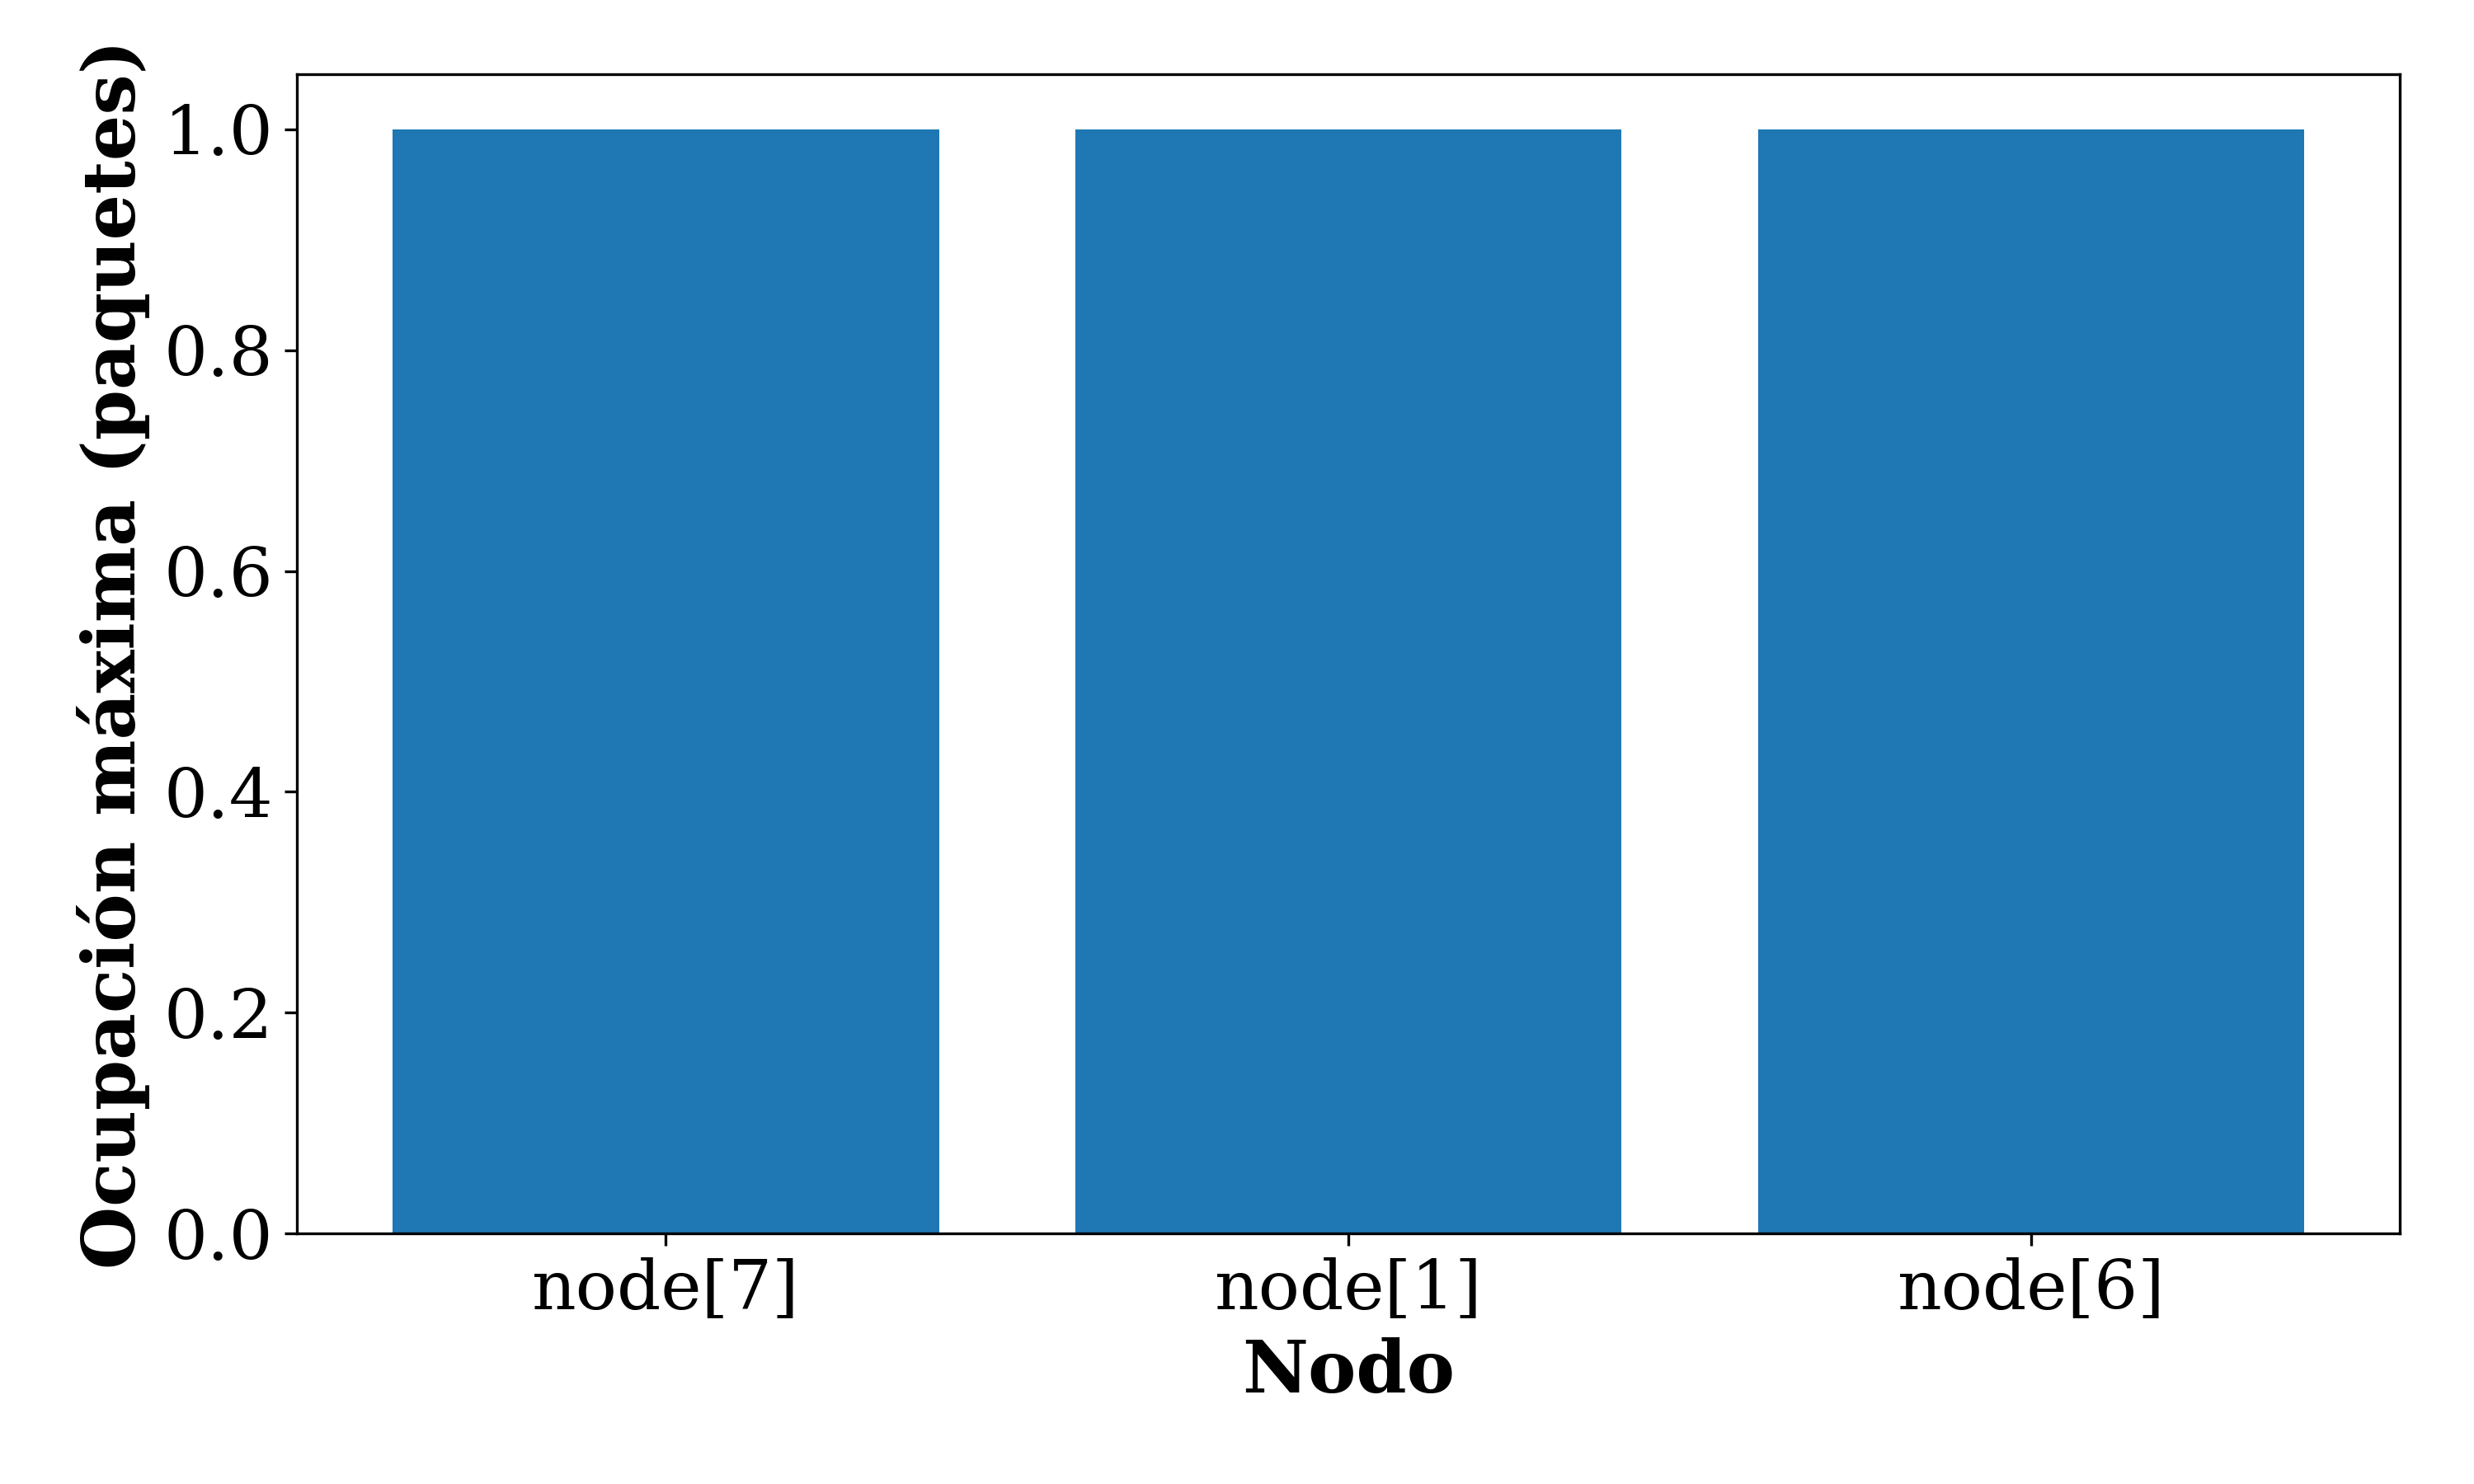
\includegraphics[width=\columnwidth]{../../figuras/entrega-parcial-caso1_buffers_intermediarios.png}
 \caption{Ocupación máxima de buffers --- nodos intermediarios (node[1], node[6] y node[7]).}
 \label{fig:entrega-parcial-caso1_buffers_intermediarios}
\end{figure}

\begin{figure}[!ht]
 \centering
 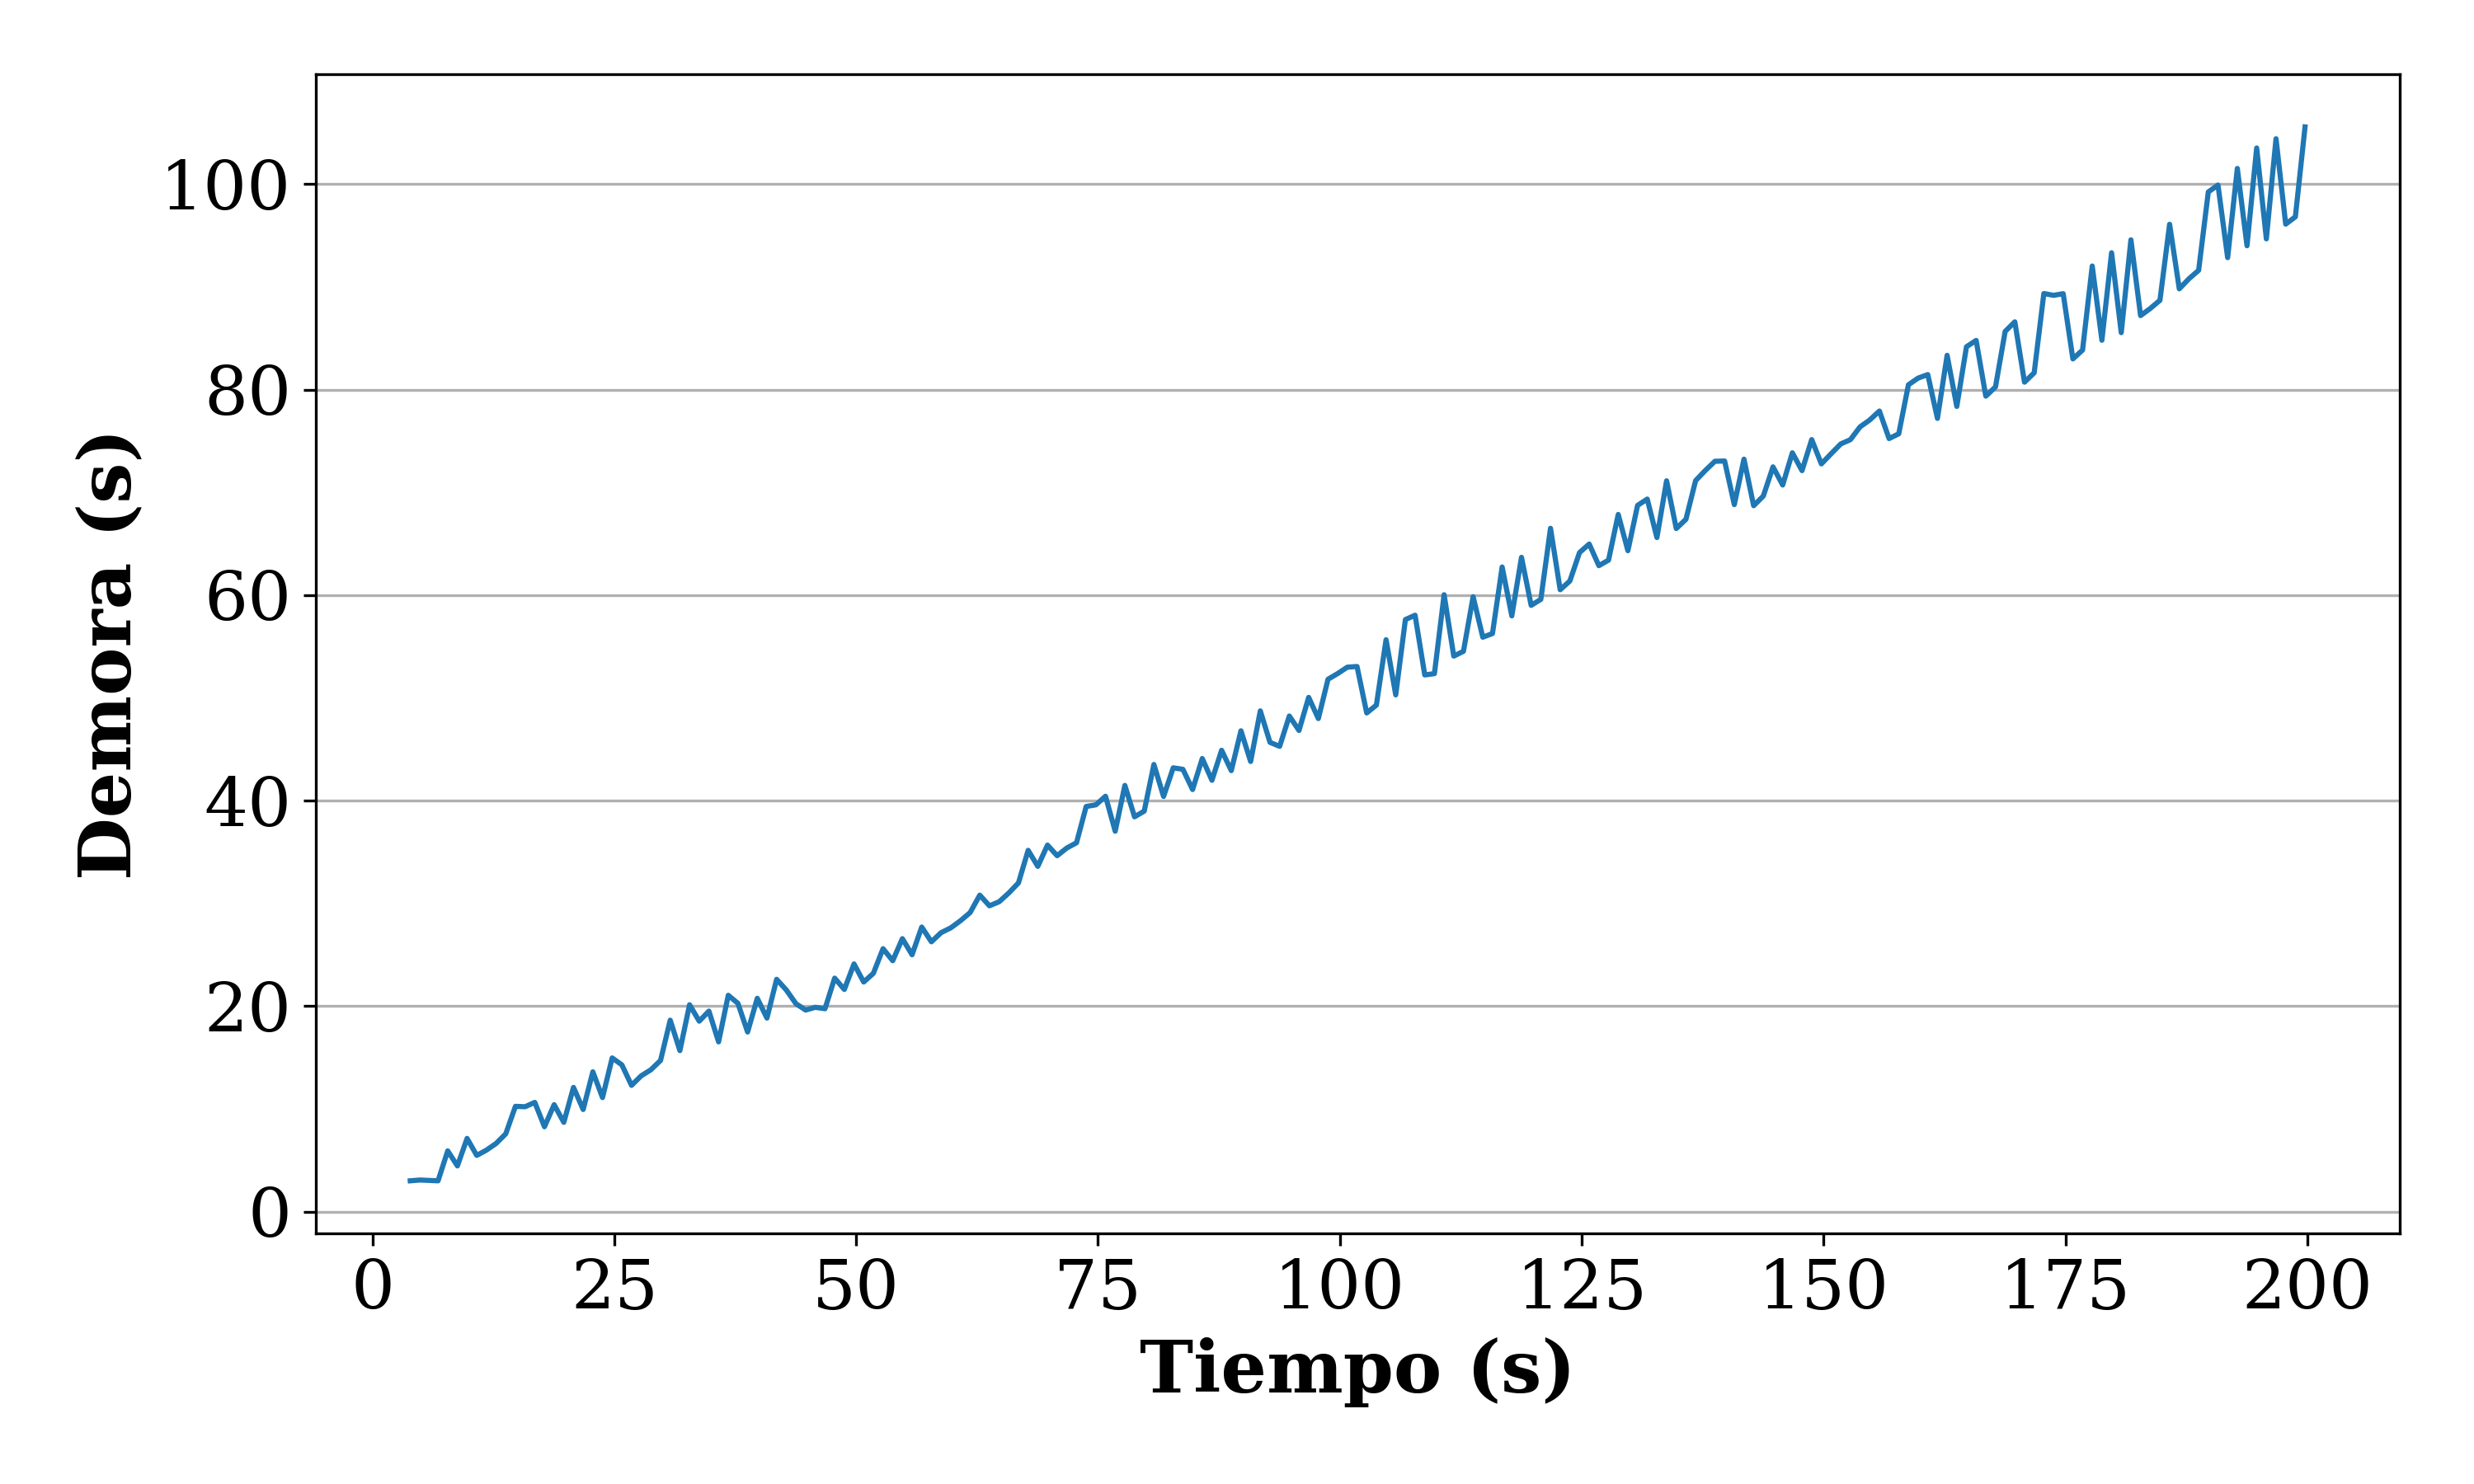
\includegraphics[width=\columnwidth]{../../figuras/entrega-parcial-caso1_delay.png}
 \caption{Demora extremo a extremo a lo largo del tiempo --- node[5].}
 \label{fig:entrega-parcial-caso1_delay}
\end{figure}

\begin{figure}[!ht]
 \centering
 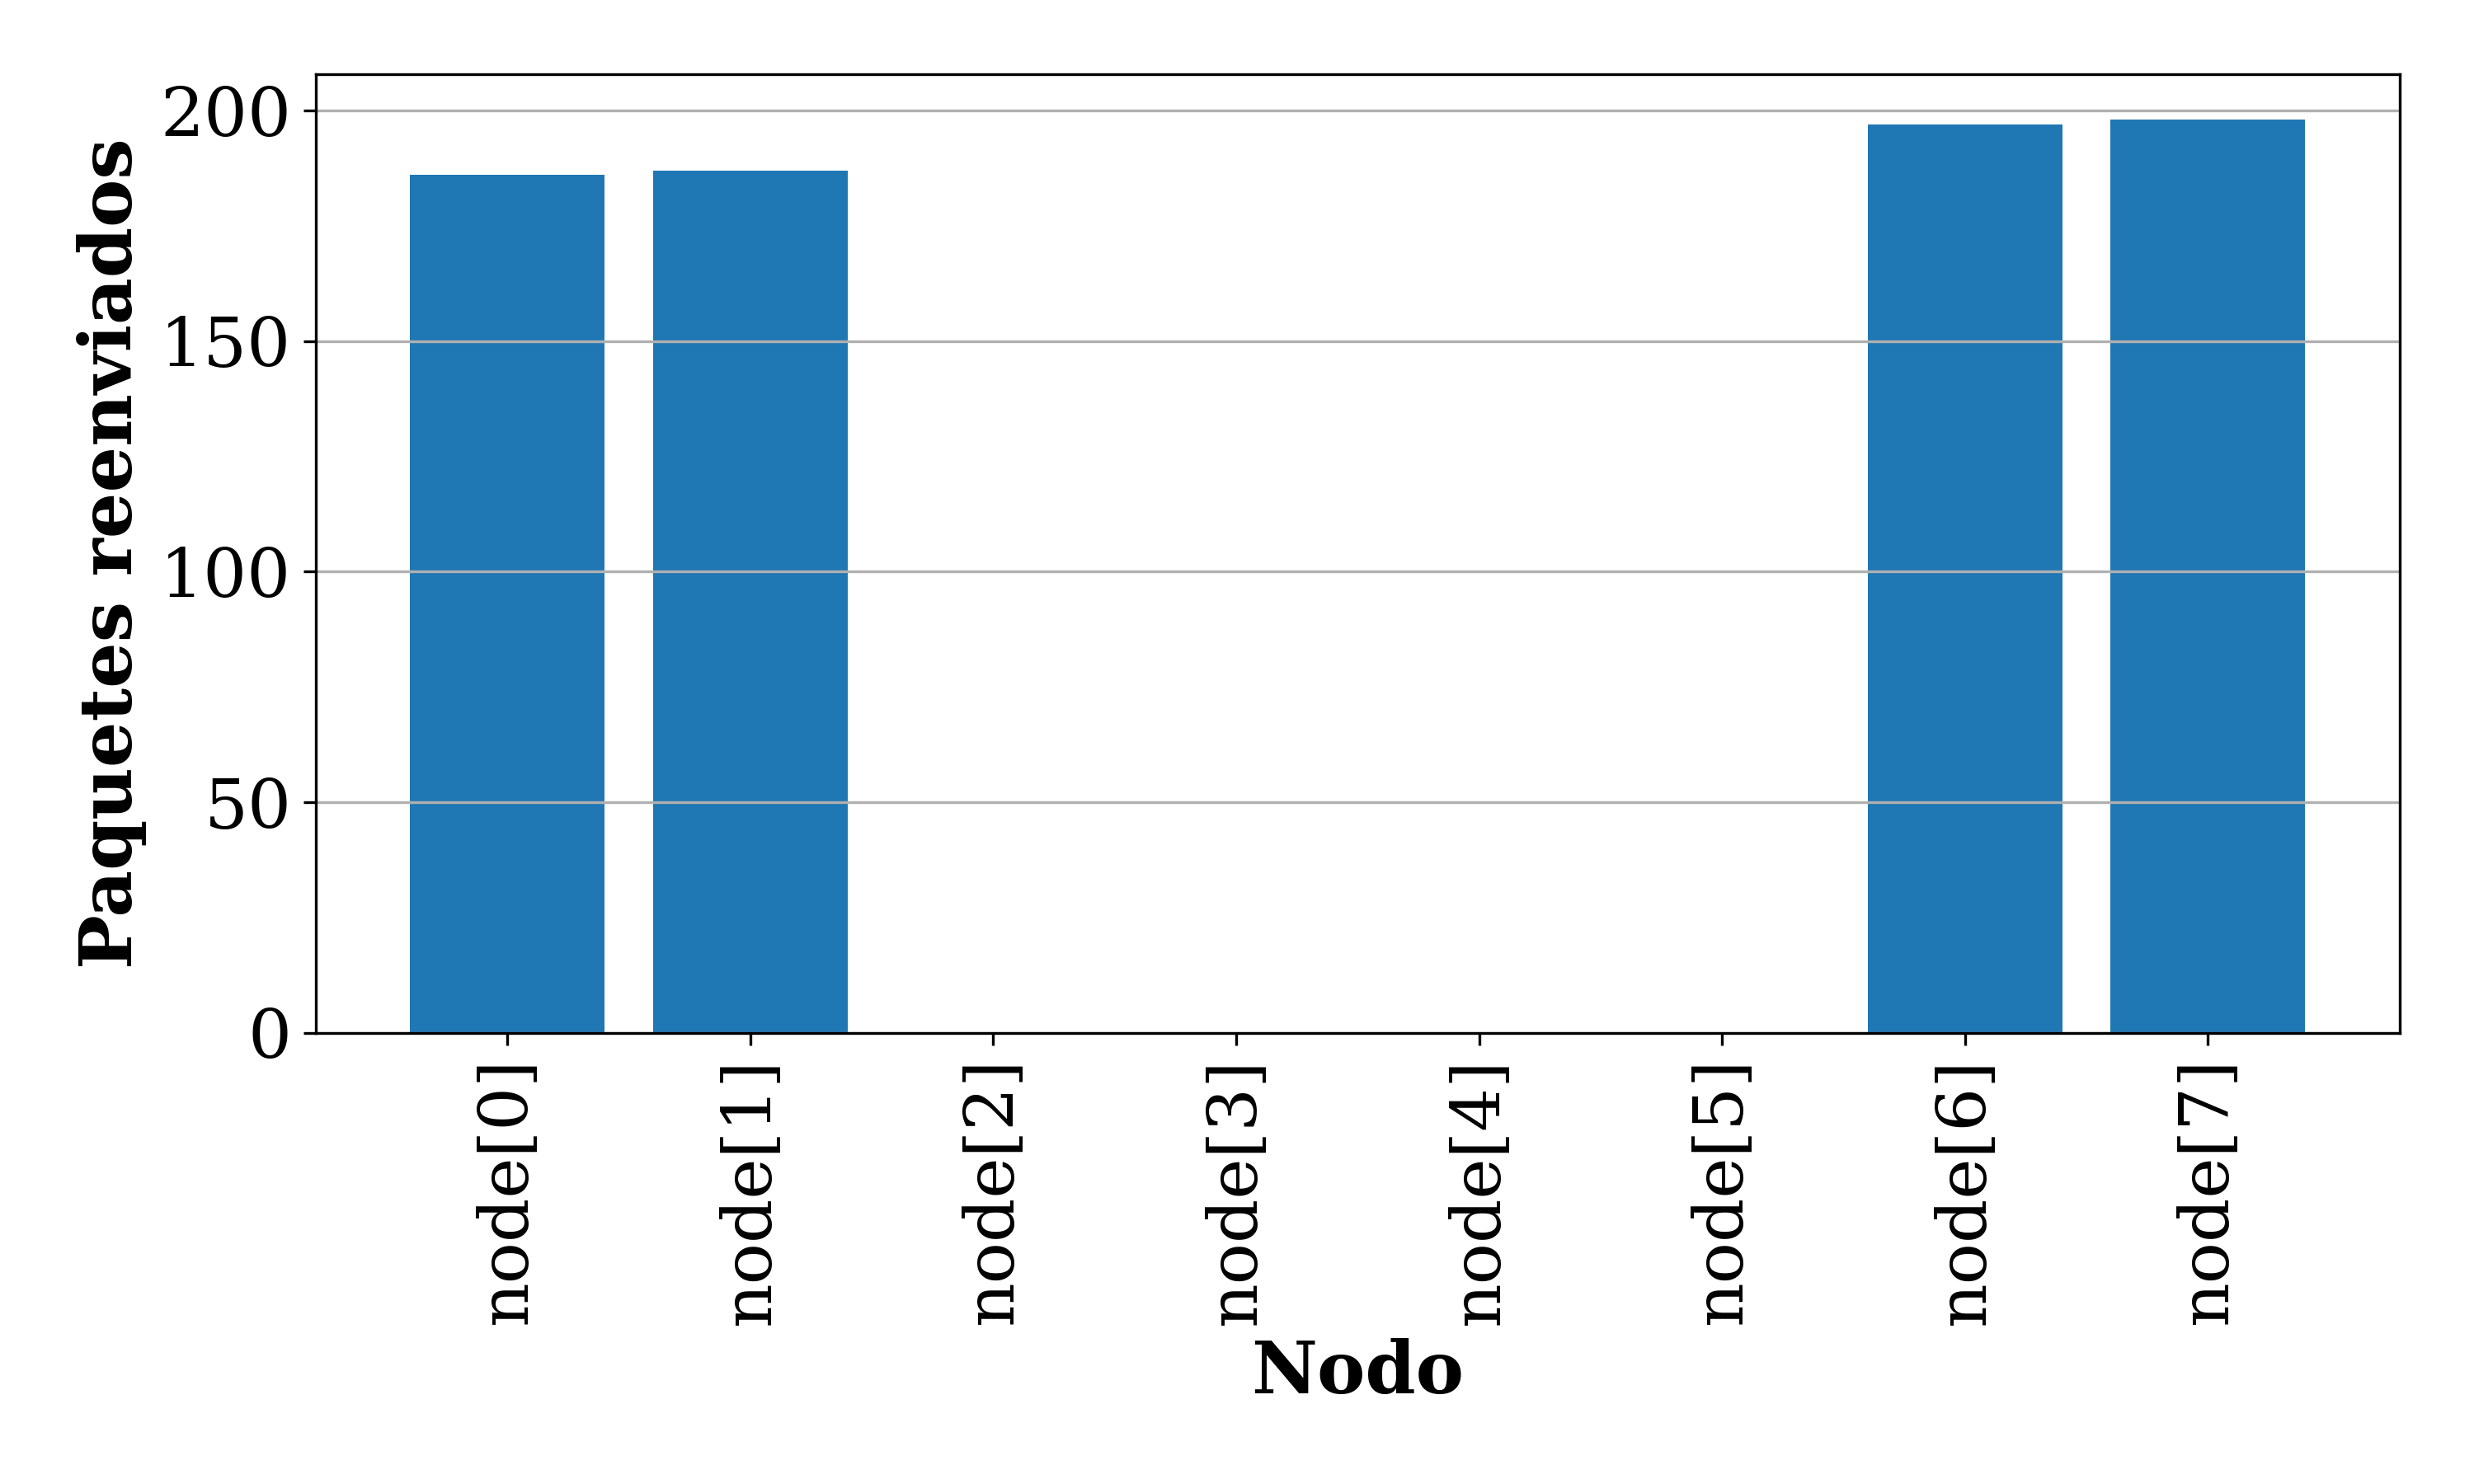
\includegraphics[width=\columnwidth]{../../figuras/entrega-parcial-caso1_forwarded.png}
 \caption{Paquetes reenviados por nodo durante la simulación.}
 \label{fig:entrega-parcial-caso1_forwarded}
\end{figure}

\textbf{\textit{Posibilidades de mejora.}} El rendimiento puede mejorarse. El algoritmo actual ignora que cada nodo dispone de dos interfaces y que existen dos caminos posibles hacia cualquier destino. Al forzar siempre el uso de \texttt{lnk[0]}, se concentra todo el tráfico en un subconjunto de enlaces, dejando la mitad de la capacidad de la red completamente sin utilizar. Esto genera saturación en los enlaces más transitados y demoras crecientes, como se observa en la Fig.~\ref{fig:entrega-parcial-caso1_delay}.

\FloatBarrier

\subsection{Caso 2: tráfico sostenido hacia \texttt{node[5]}}

A partir de \texttt{interArrivalTime} = 7\,s la red permanece estable porque los buffers de todos los nodos se mantienen acotados a lo largo de la simulación (Figs.~\ref{fig:entrega-parcial-caso2_buffers_iat05}--\ref{fig:entrega-parcial-caso2_buffers_iat5} y Tabla~\ref{tab:caso2-sweep}). Para valores menores de \texttt{interArrivalTime}, al menos un buffer crece indefinidamente, lo que evidencia saturación.

La estabilización de la red a partir de \texttt{iat}=7 también se refleja en la demora media (Fig.~\ref{fig:entrega-parcial-caso2-estabilidad}), que cae drásticamente de 34\,s a 7\,s entre \texttt{iat}=5 y \texttt{iat}=7, y se mantiene en valores bajos para valores mayores de \texttt{iat}.

\begin{figure}[!ht]
  \centering
  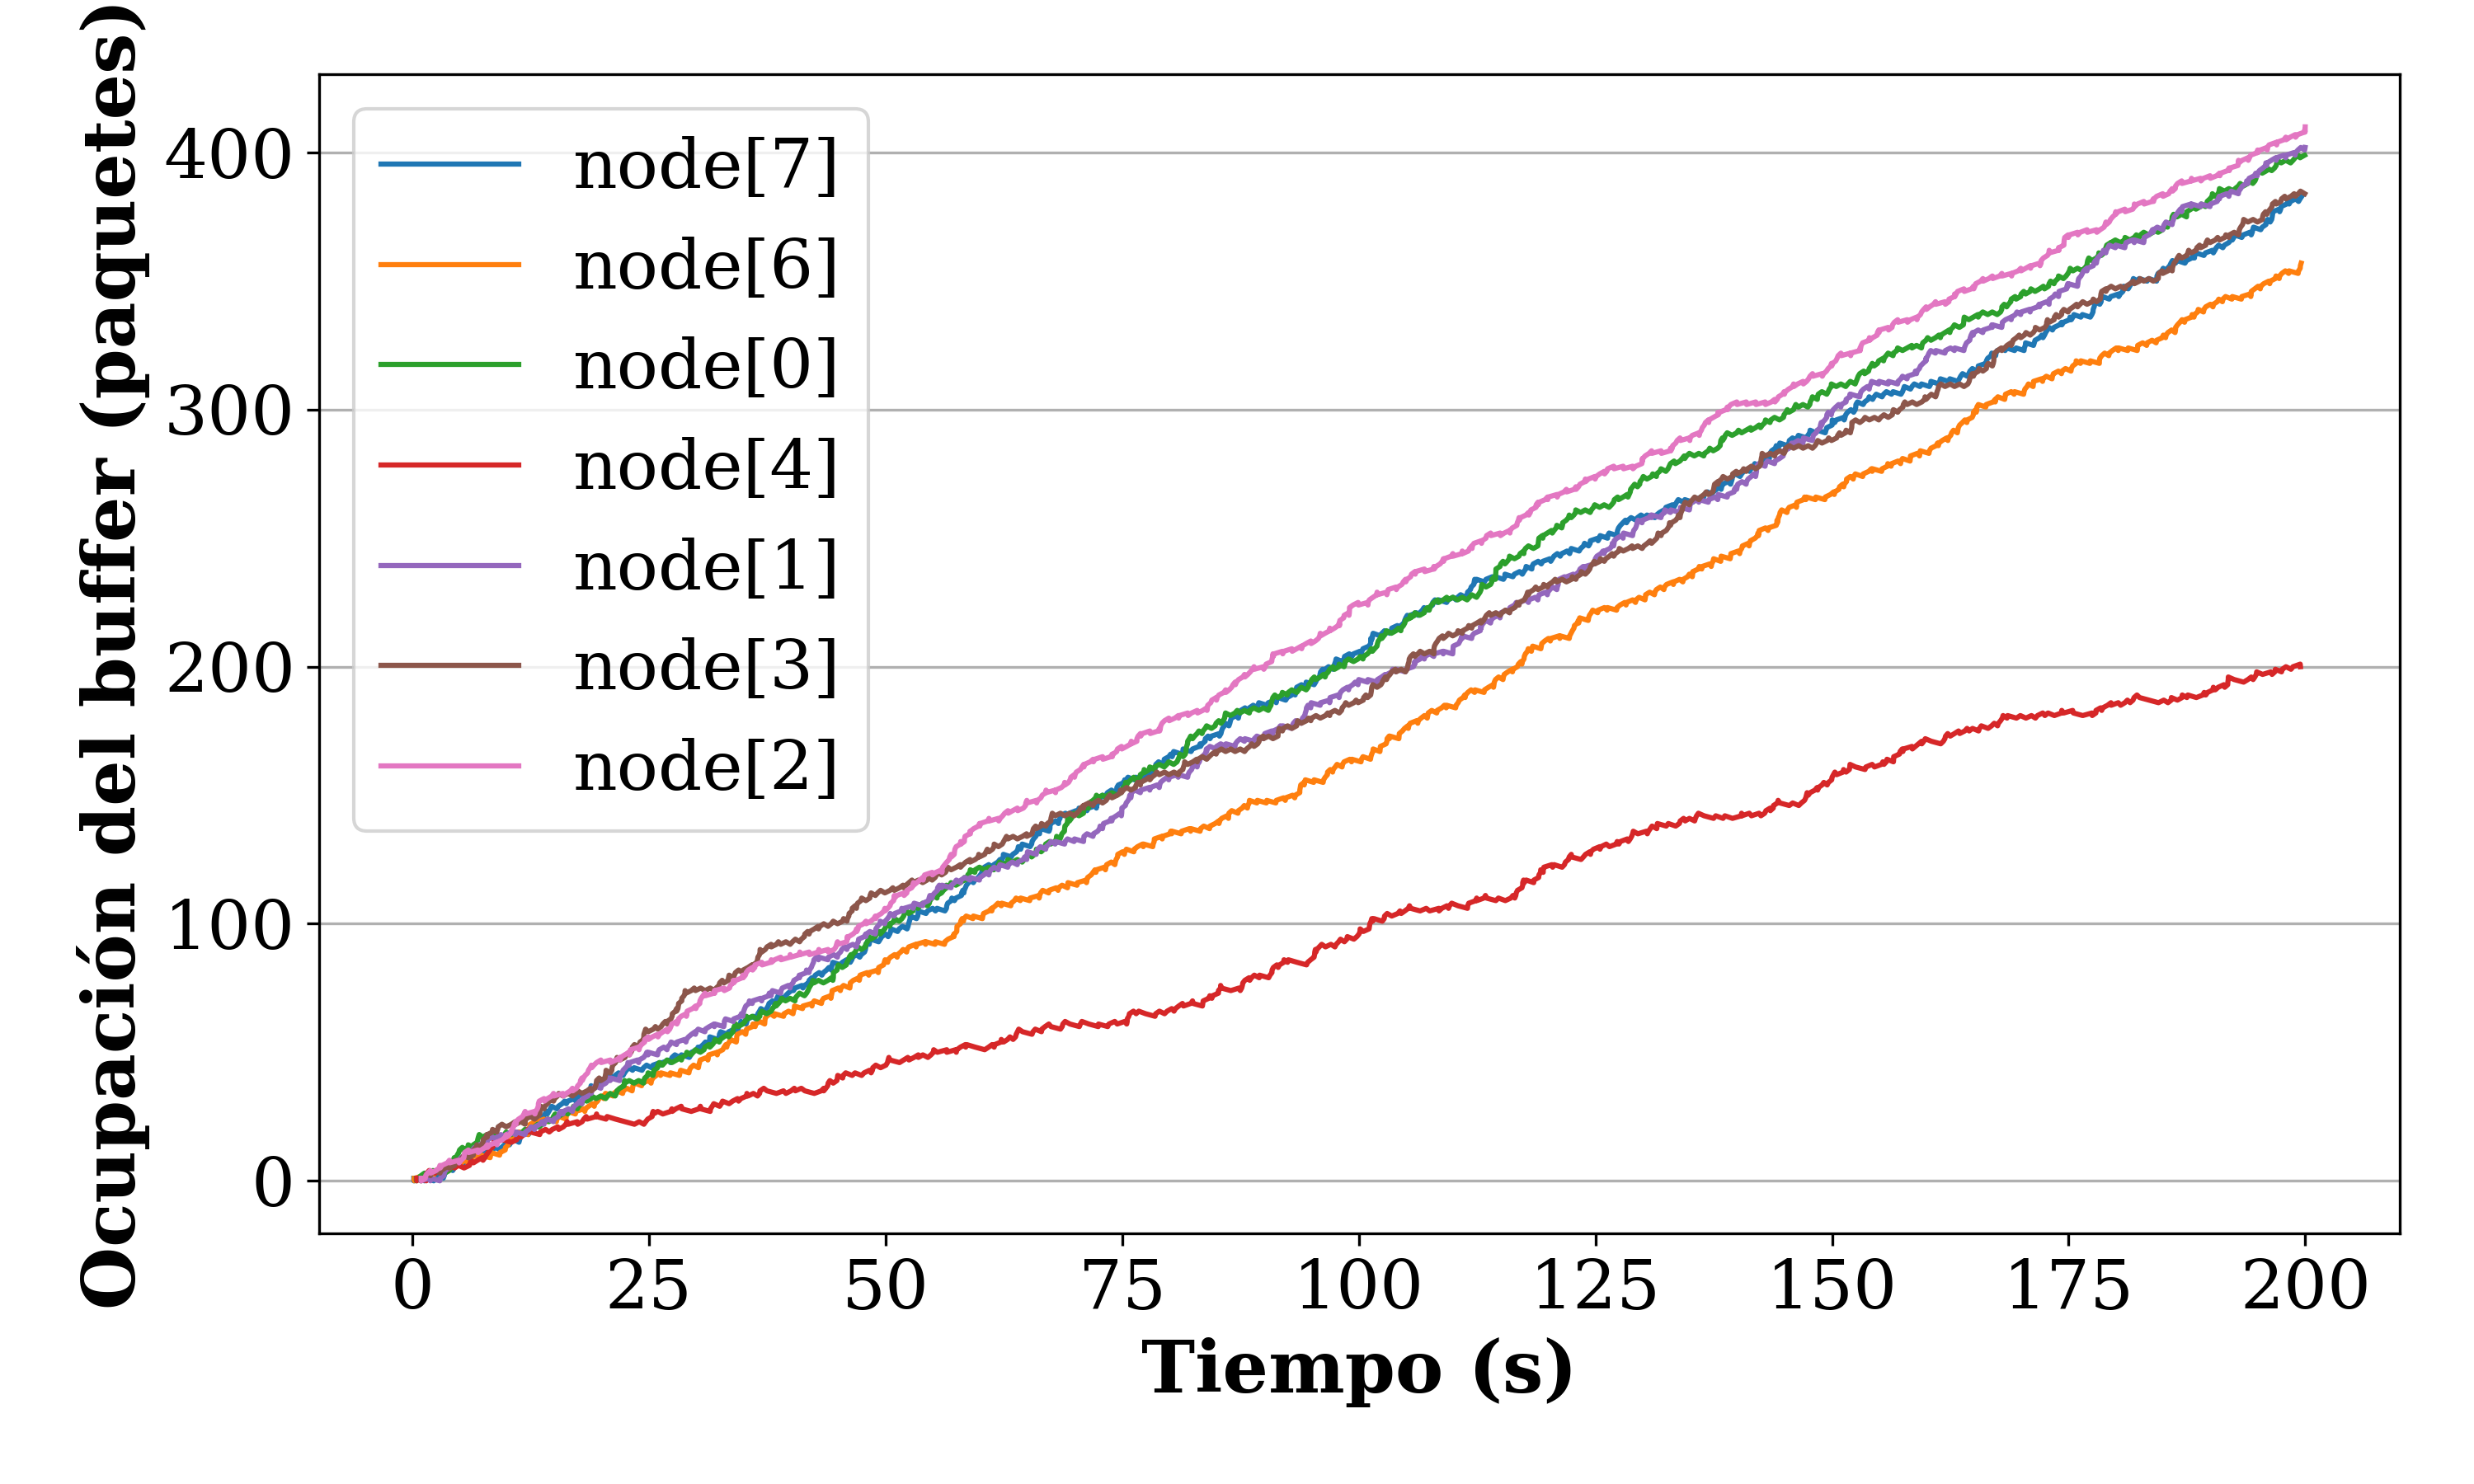
\includegraphics[width=\columnwidth]{../../figuras/entrega-parcial-caso2_buffers_iat0.5.png}
  \caption{Ocupación de buffers a lo largo del tiempo --- \texttt{iat}=0.5\,s.}
  \label{fig:entrega-parcial-caso2_buffers_iat05}
\end{figure}

\begin{figure}[!ht]
  \centering
  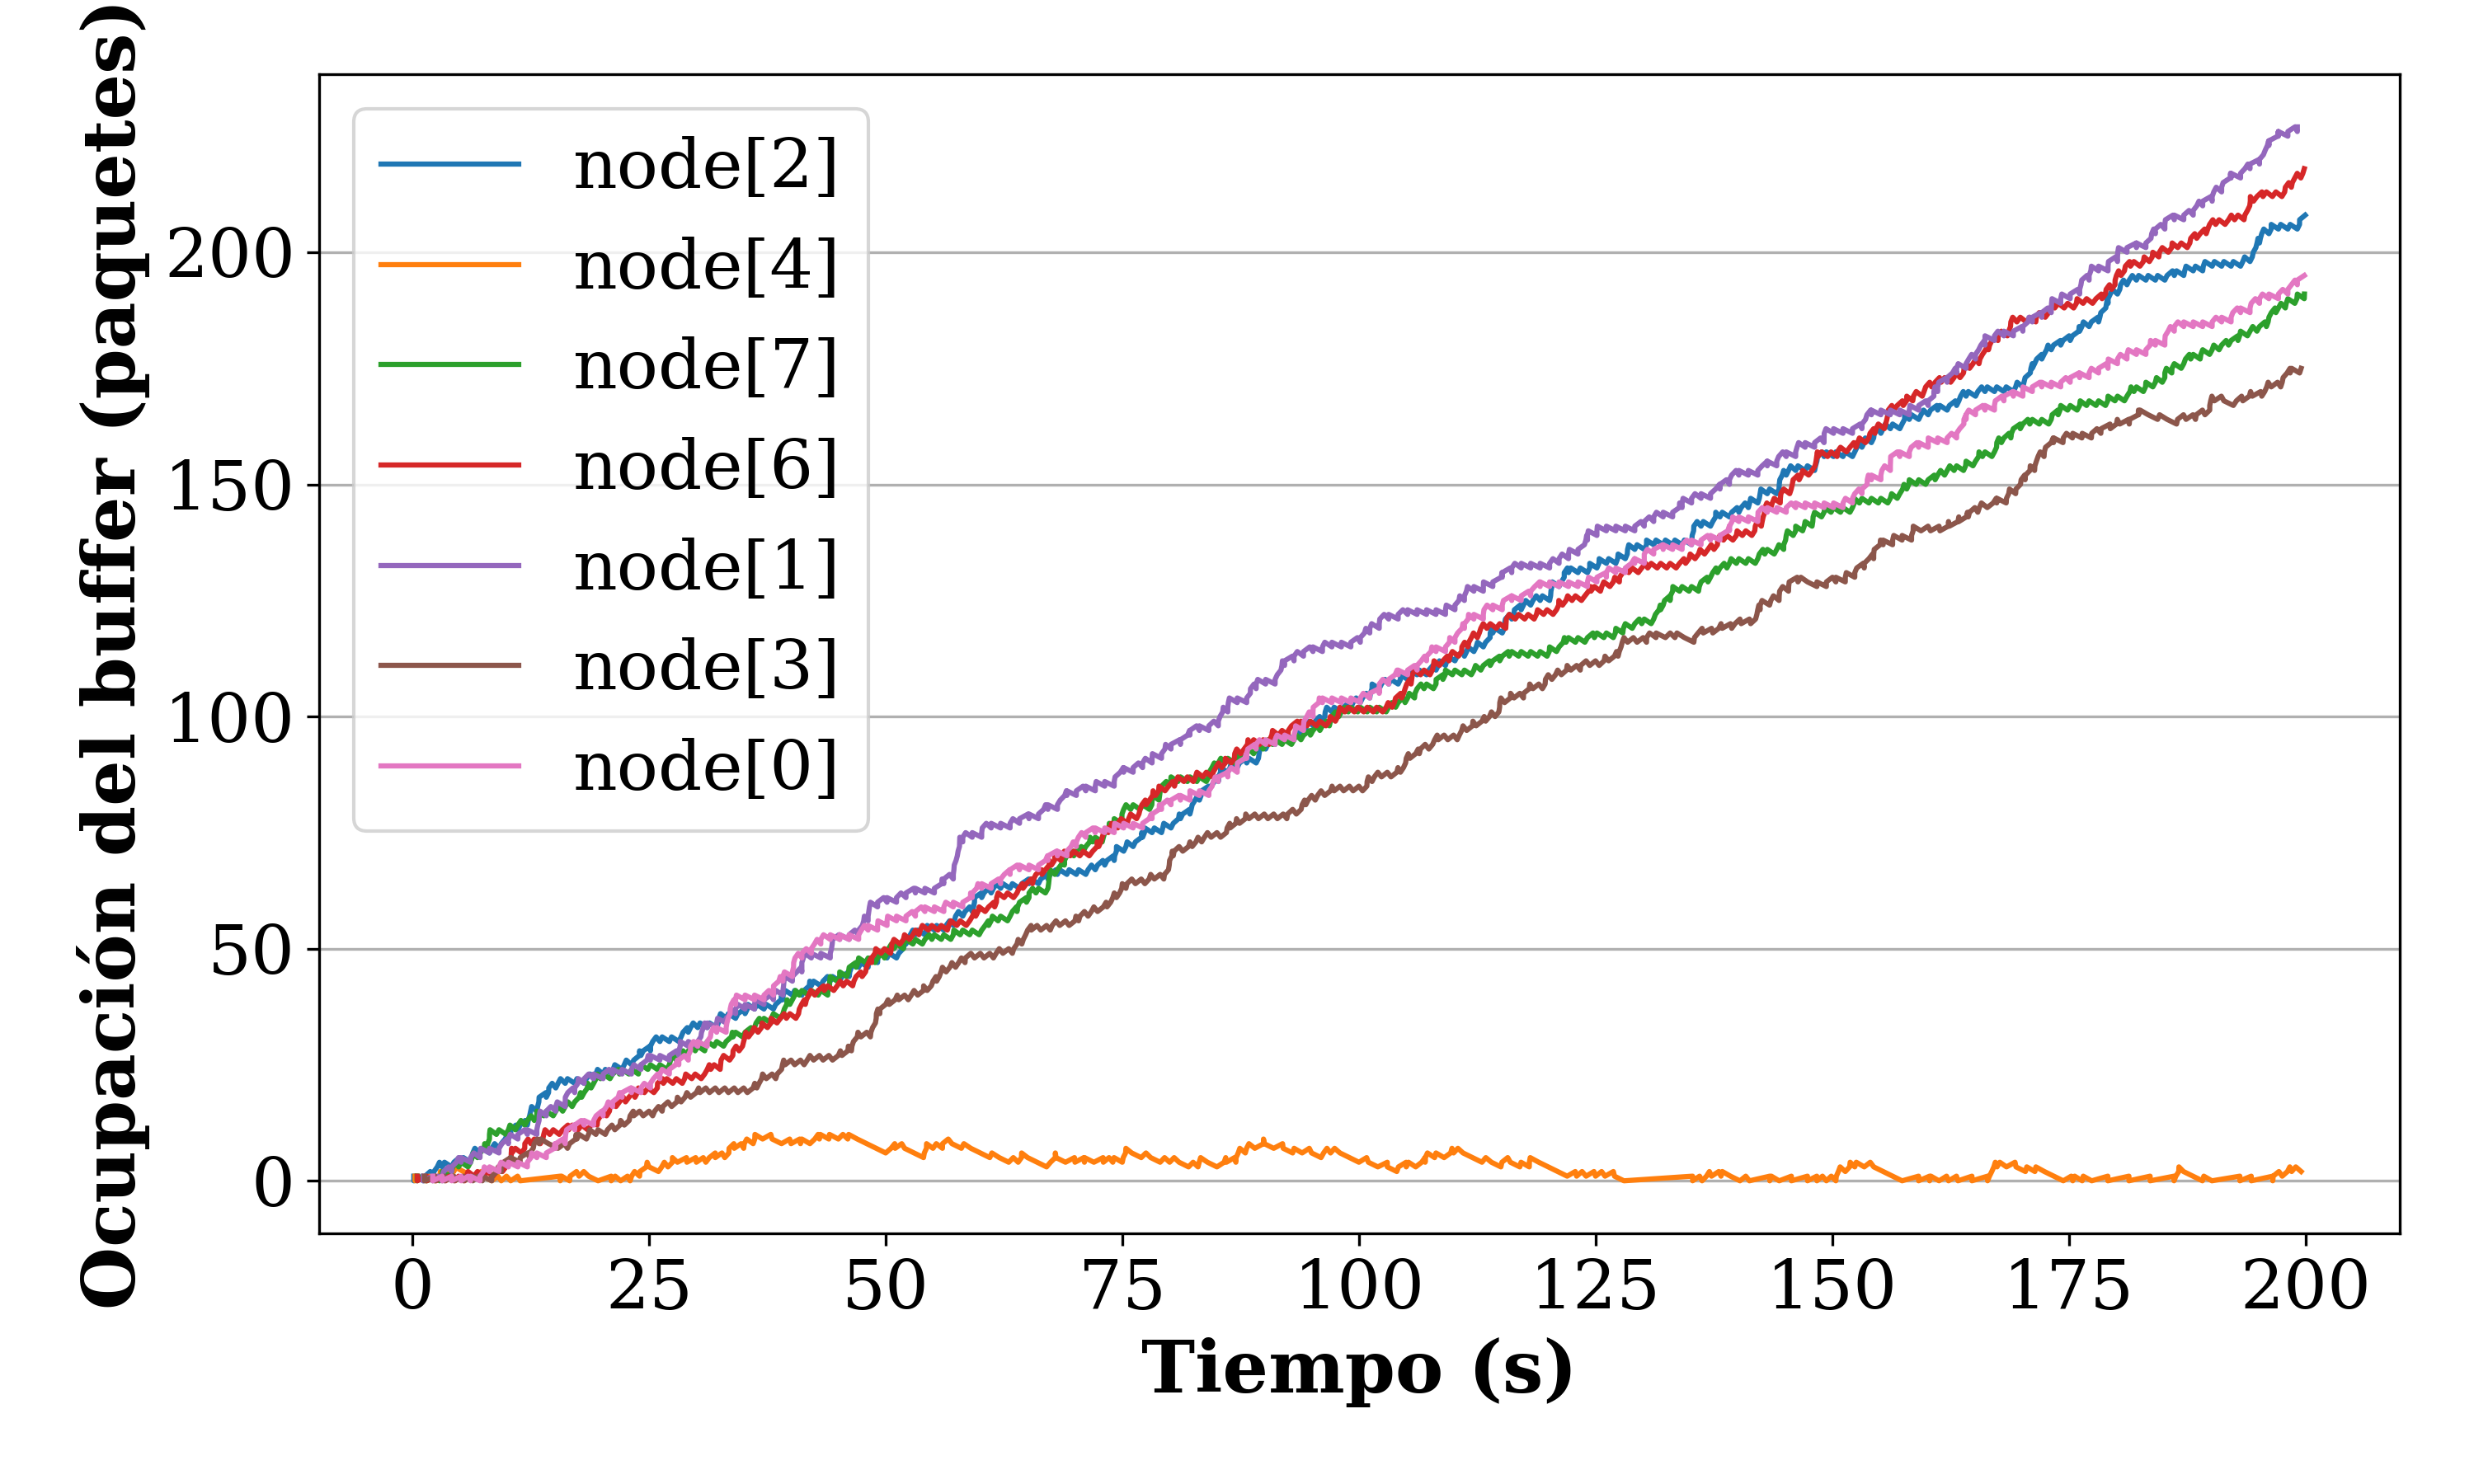
\includegraphics[width=\columnwidth]{../../figuras/entrega-parcial-caso2_buffers_iat1.png}
  \caption{Ocupación de buffers a lo largo del tiempo --- \texttt{iat}=1\,s.}
  \label{fig:entrega-parcial-caso2_buffers_iat1}
\end{figure}

\begin{figure}[!ht]
  \centering
  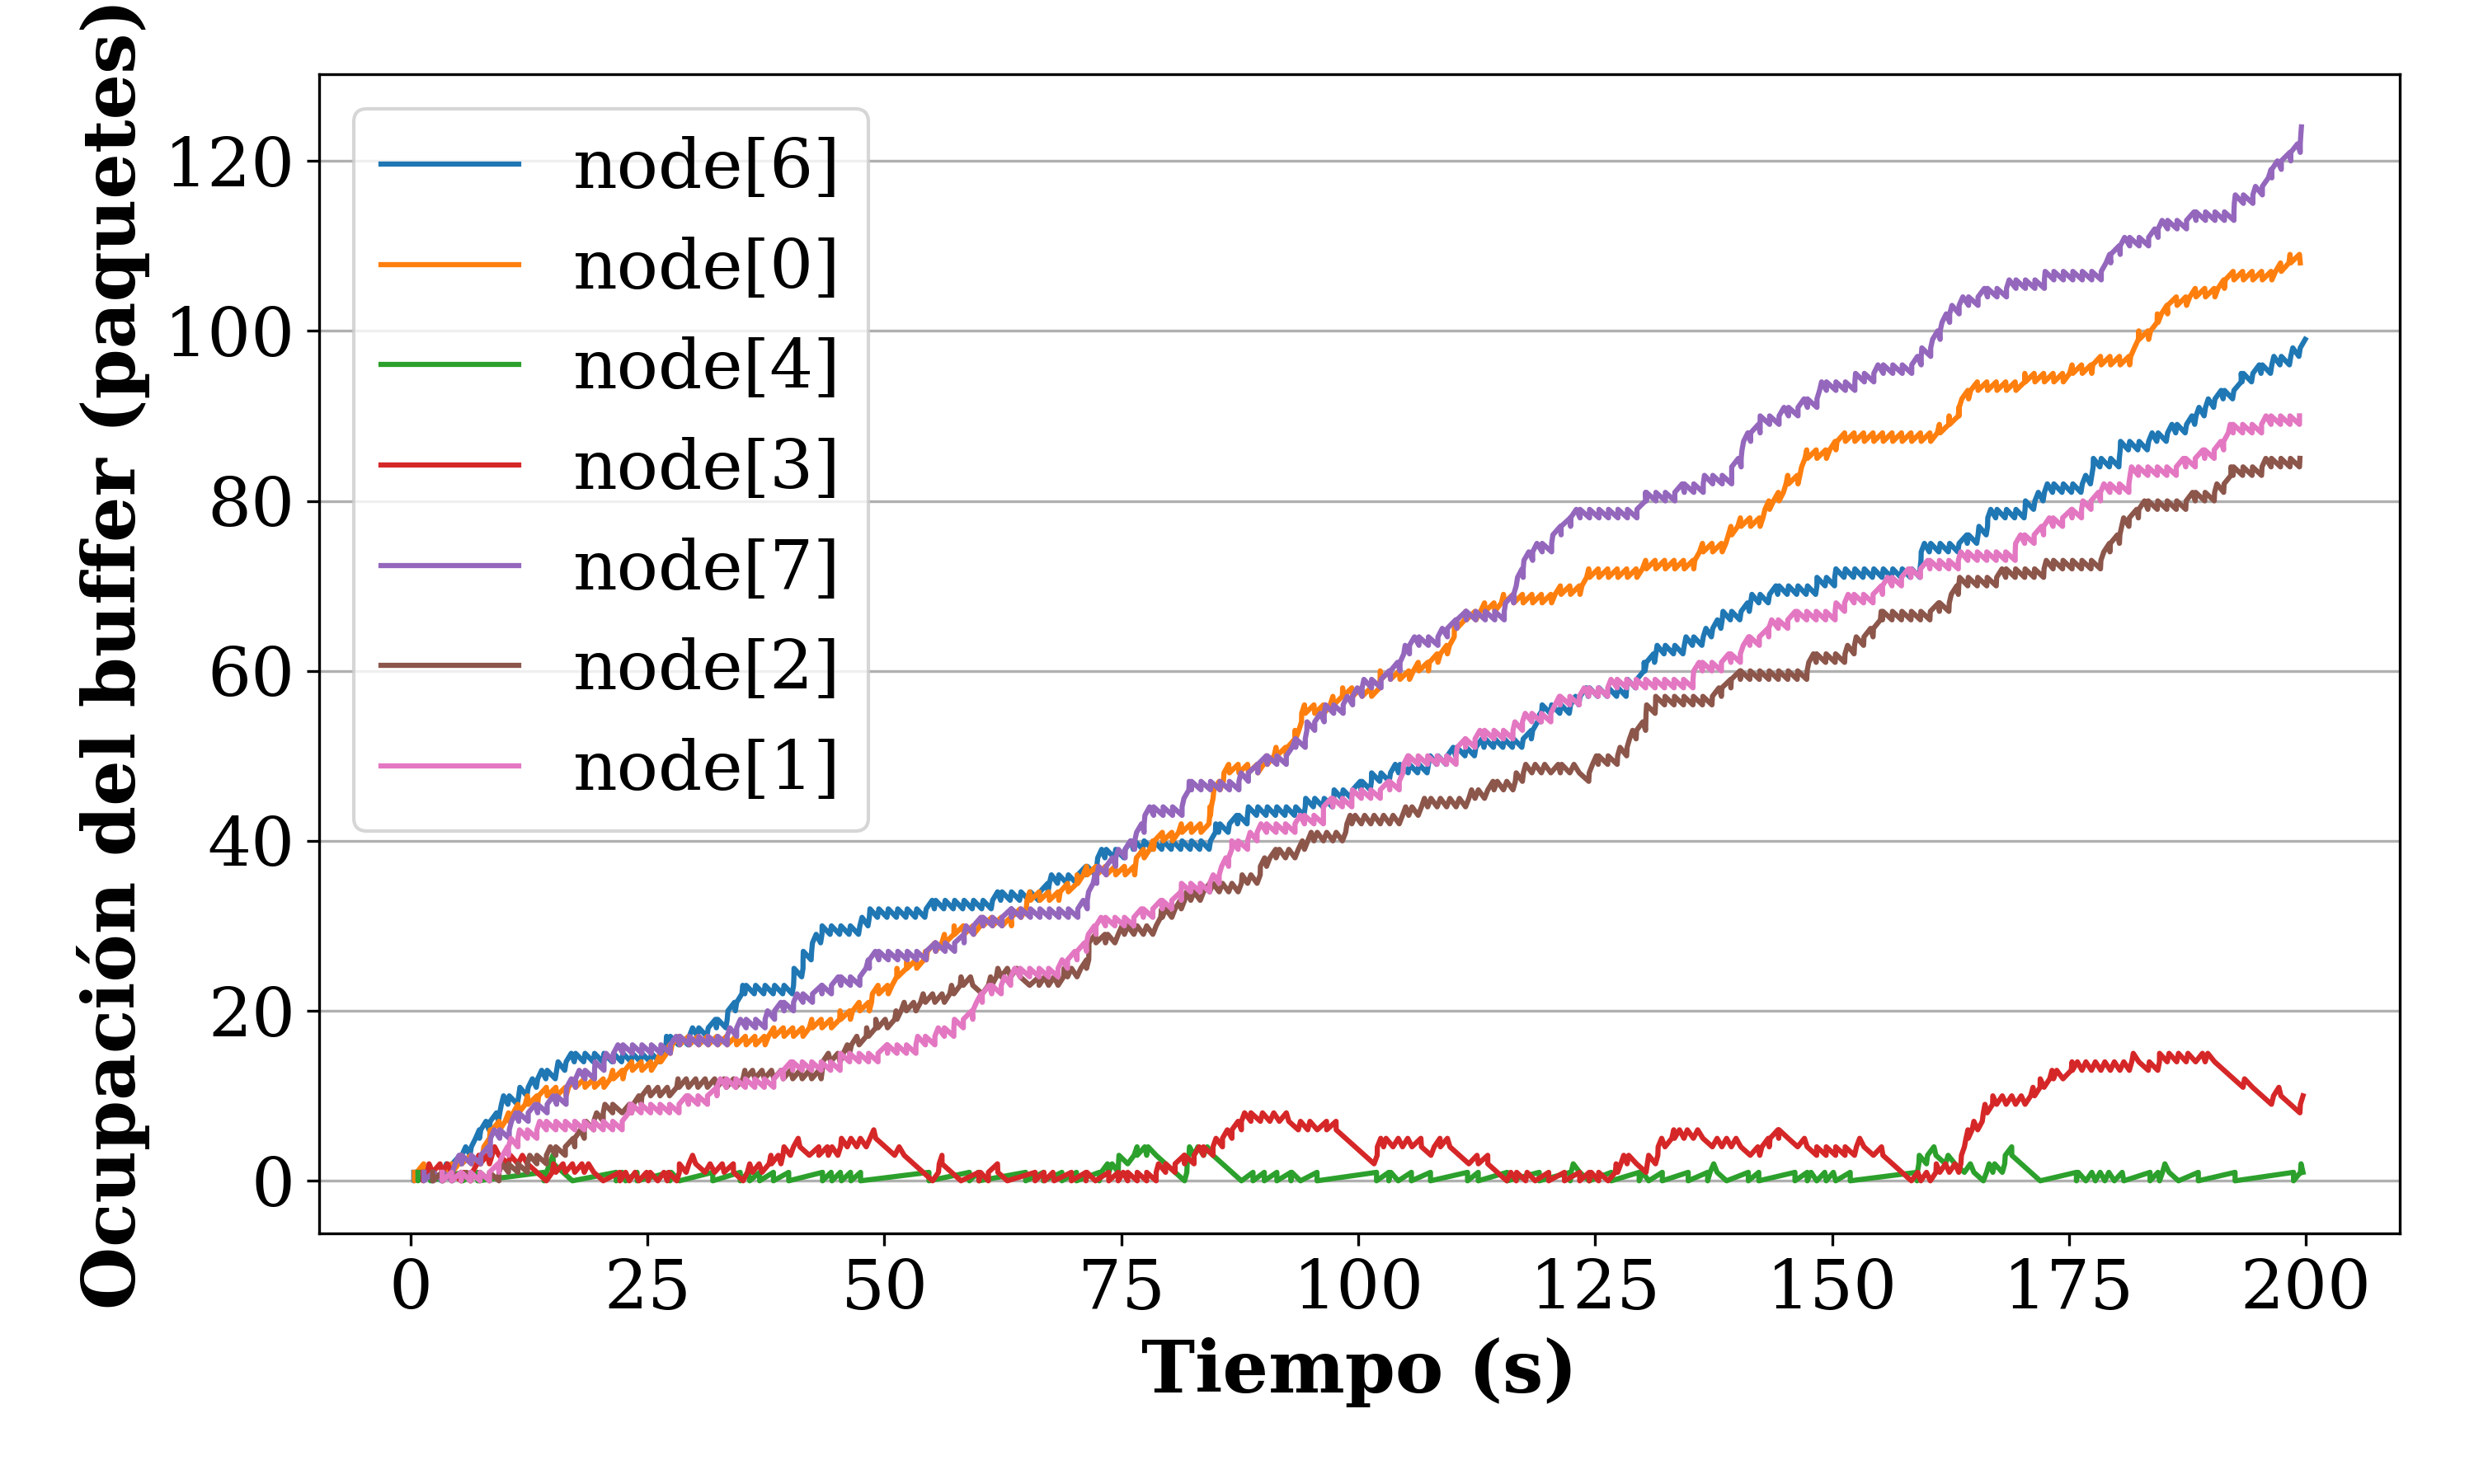
\includegraphics[width=\columnwidth]{../../figuras/entrega-parcial-caso2_buffers_iat2.png}
  \caption{Ocupación de buffers a lo largo del tiempo --- \texttt{iat}=2\,s.}
  \label{fig:entrega-parcial-caso2_buffers_iat2}
\end{figure}

\begin{figure}[!ht]
  \centering
  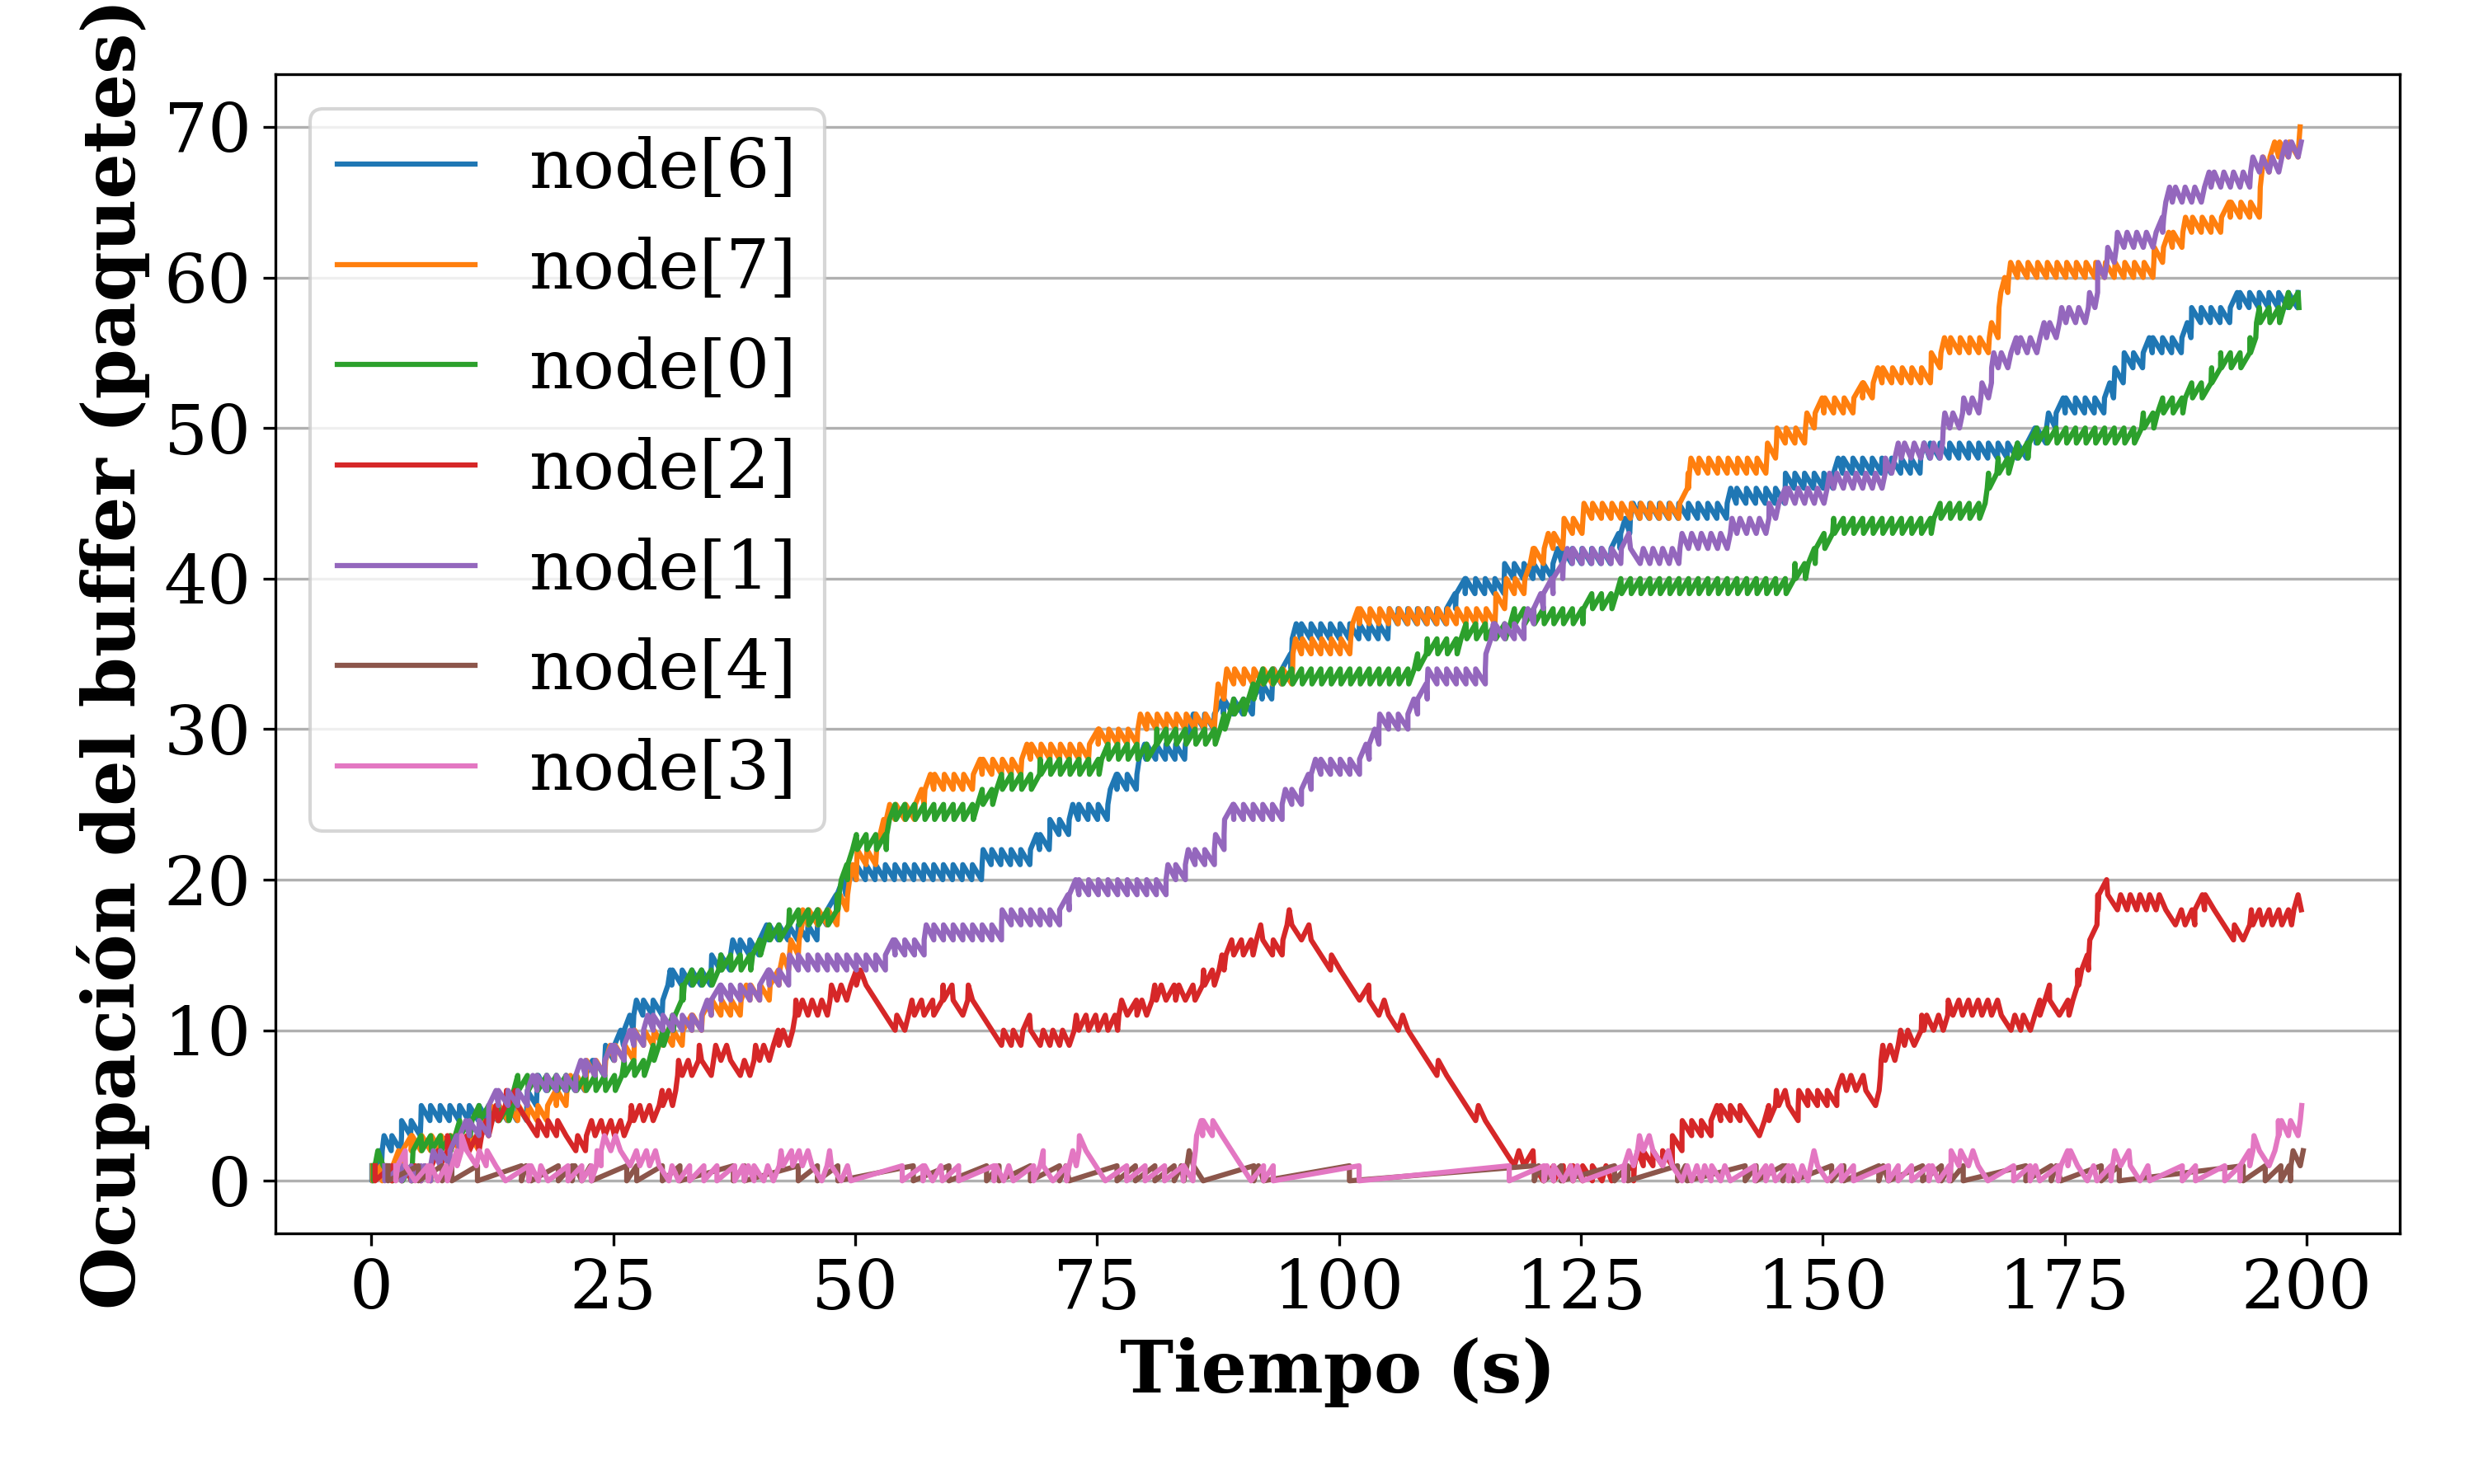
\includegraphics[width=\columnwidth]{../../figuras/entrega-parcial-caso2_buffers_iat3.png}
  \caption{Ocupación de buffers a lo largo del tiempo --- \texttt{iat}=3\,s.}
  \label{fig:entrega-parcial-caso2_buffers_iat3}
\end{figure}

\begin{figure}[!ht]
  \centering
  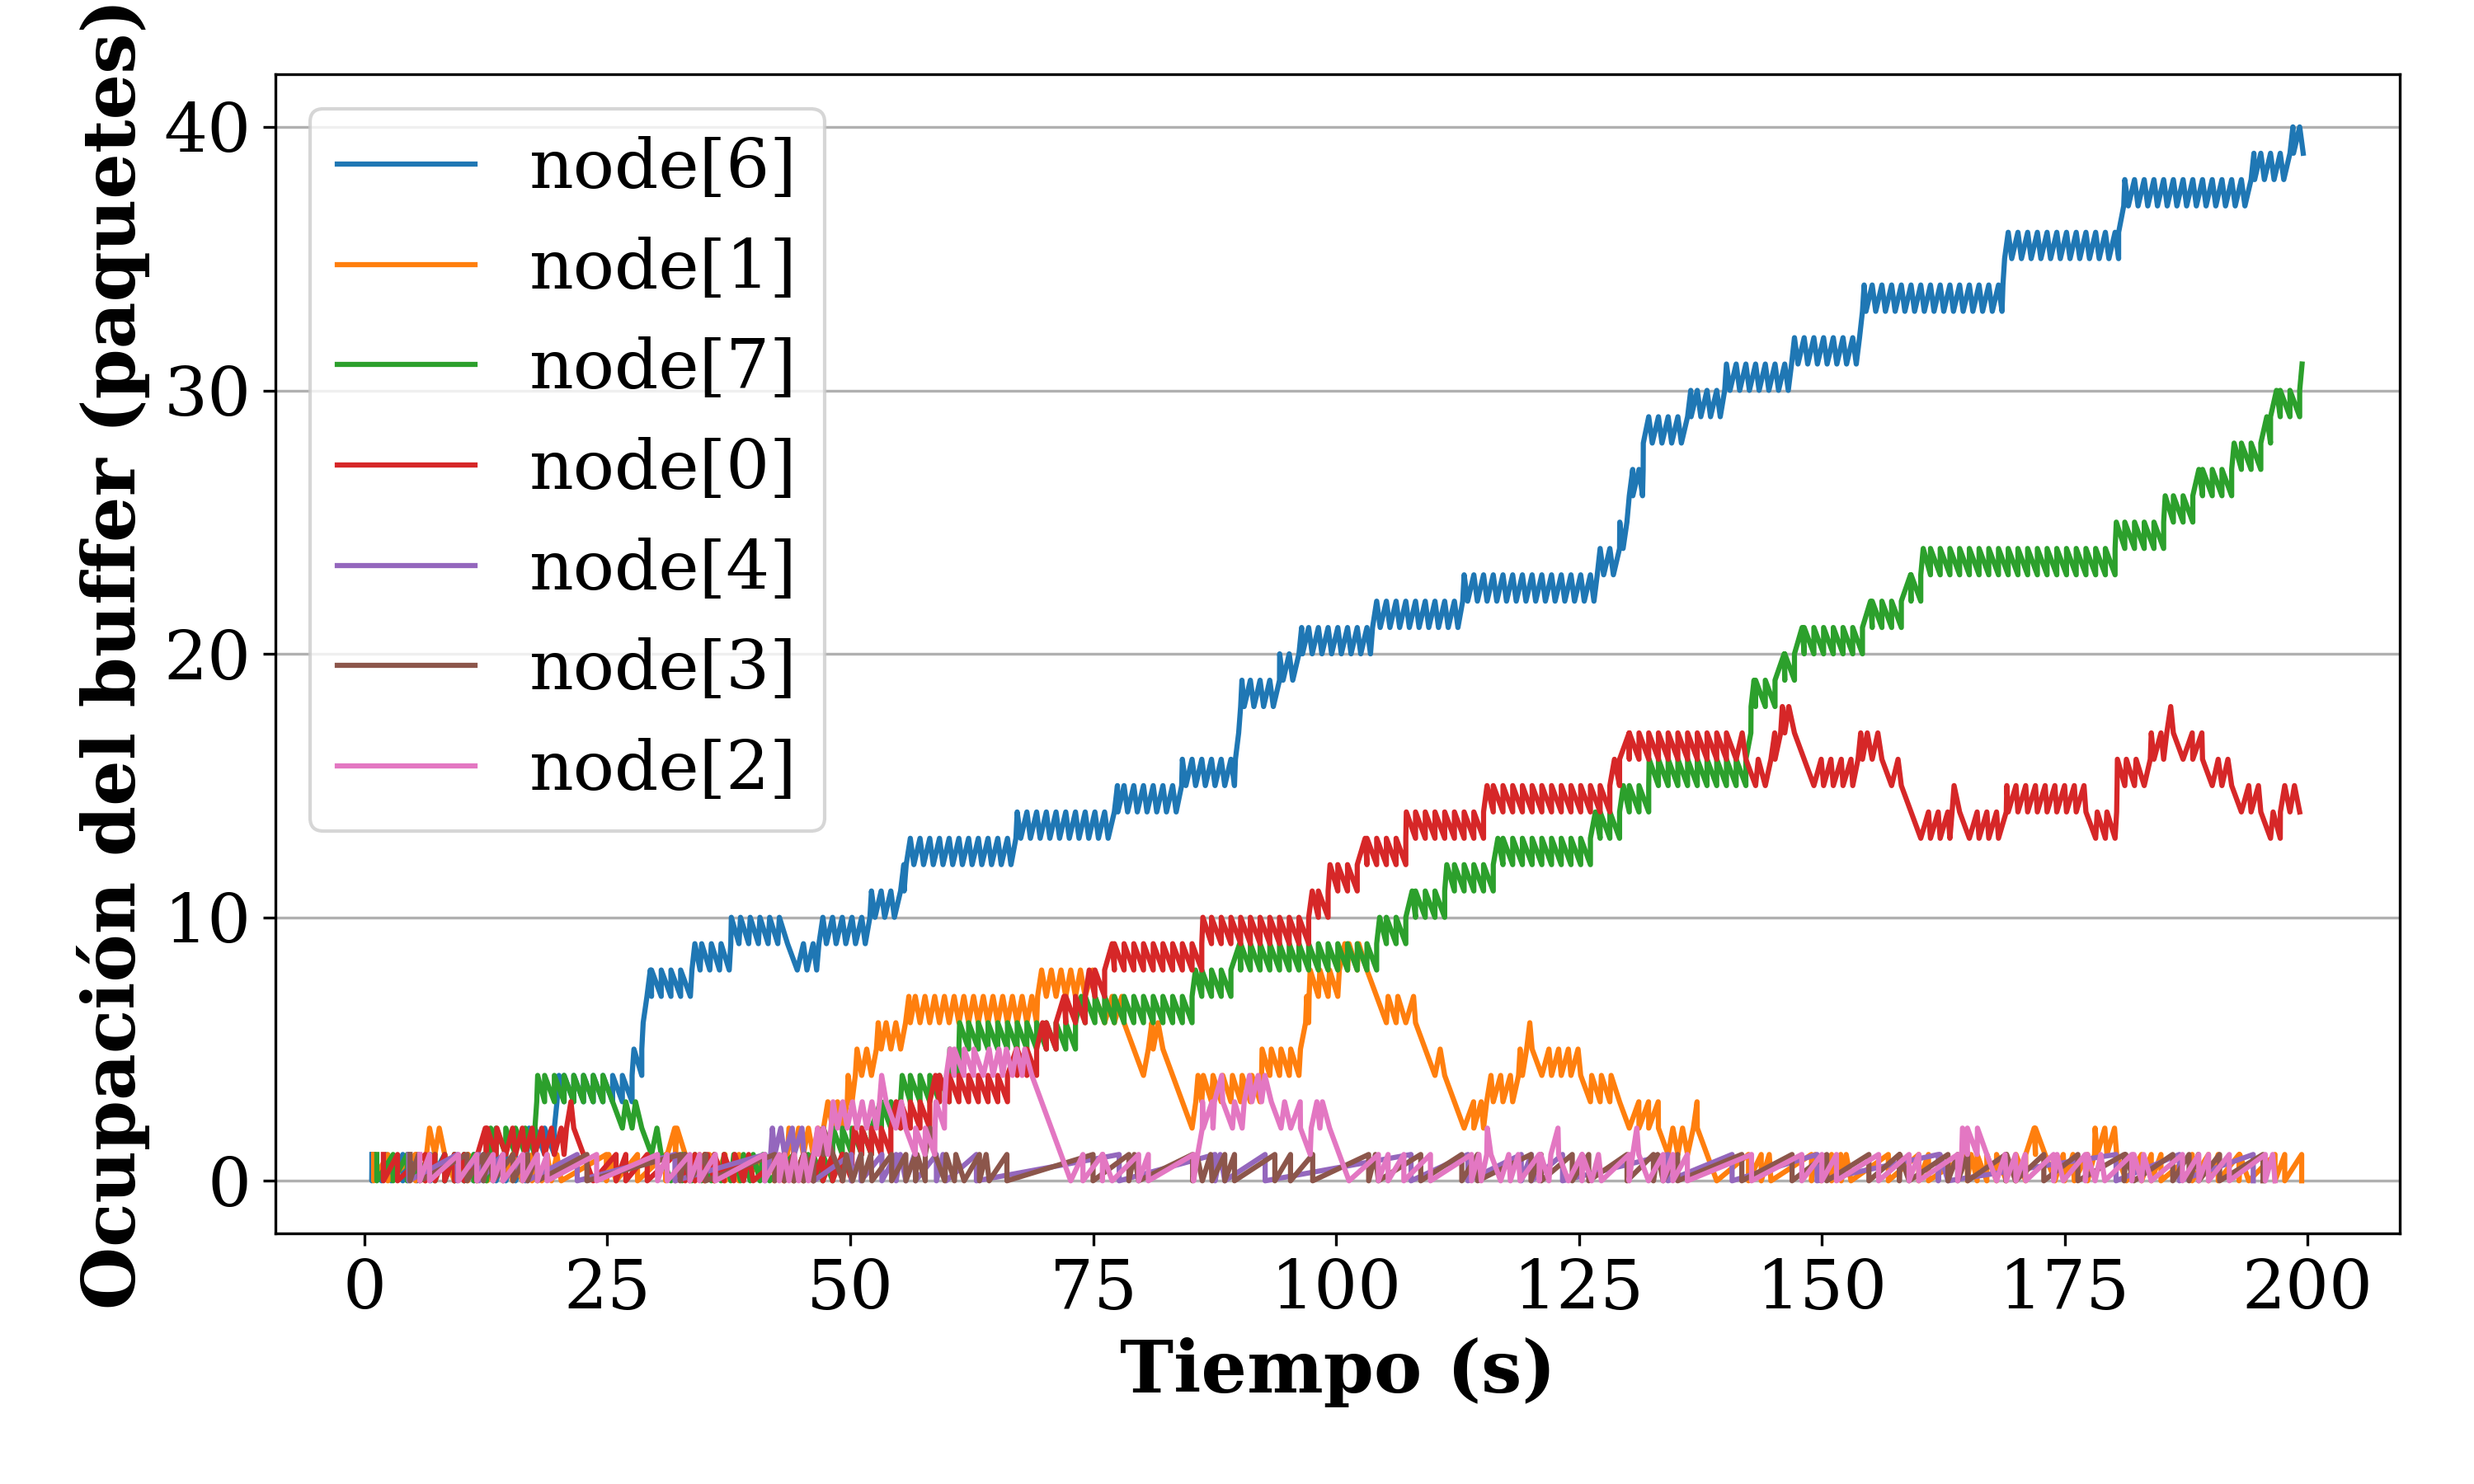
\includegraphics[width=\columnwidth]{../../figuras/entrega-parcial-caso2_buffers_iat5.png}
  \caption{Ocupación de buffers a lo largo del tiempo --- \texttt{iat}=5\,s.}
  \label{fig:entrega-parcial-caso2_buffers_iat5}
\end{figure}

\begin{figure}[!t]
  \centering
  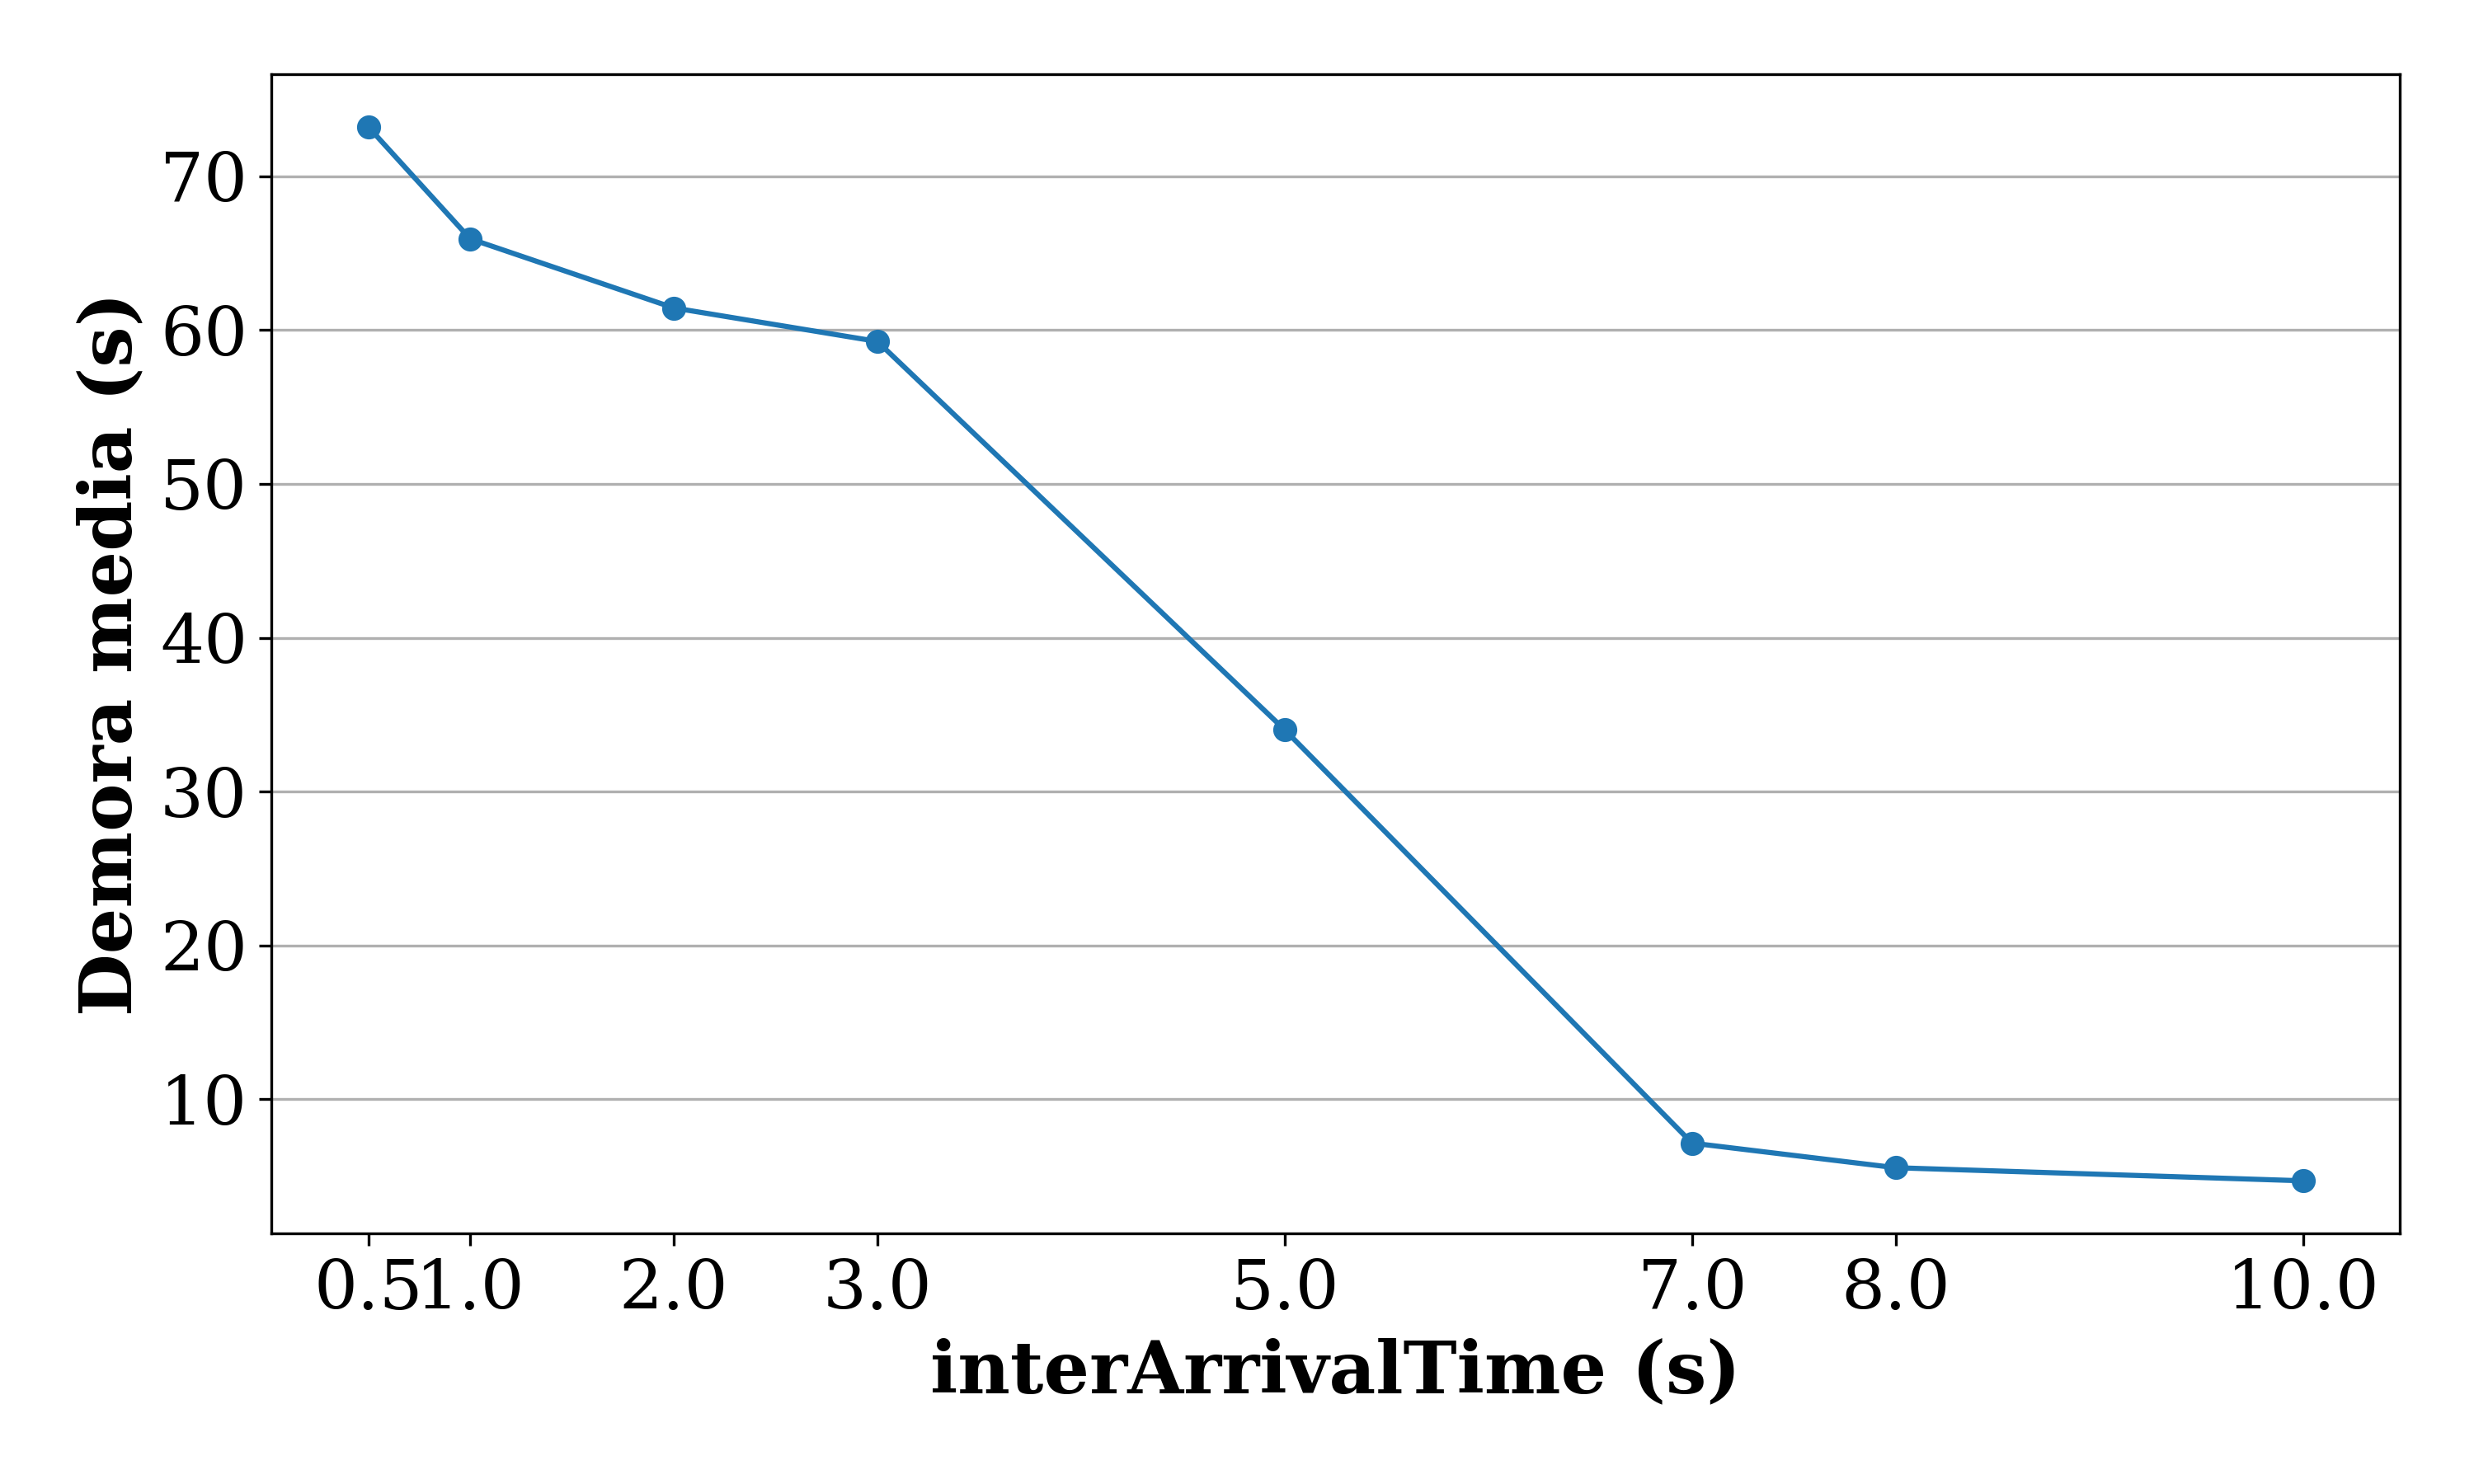
\includegraphics[width=\columnwidth]{../../figuras/entrega-parcial-caso2_delay_vs_iat.png}
  \caption{Demora media vs.\ \texttt{interArrivalTime} --- Caso 2.}
  \label{fig:entrega-parcial-caso2-estabilidad}
\end{figure}

\begin{table}[!ht]
  \centering
  \caption{Exploración del Caso~2: métricas vs.\ \texttt{interArrivalTime}.}
  \label{tab:caso2-sweep}
  \coltablesetup
  \resizebox{\columnwidth}{!}{%
  \begin{tabular}{@{}cccc@{}}
    \toprule
    \textbf{\texttt{interArriv.}} & \textbf{Demora (s)} & \textbf{Ocup. buffer máx.} & \textbf{Estab.} \\
    \midrule
    0.5 & 73.19 & 410 & No \\
    1.0 & 65.92 & 227 & No \\
    2.0 & 61.43 & 124 & No \\
    3.0 & 59.25 &  70 & No \\
    5.0 & 34.01 &  40 & No \\
    7.0 &  7.16 &   4 & Sí \\
    8.0 &  5.56 &   4 & Sí \\
    10.0 & 4.71 &   2 & Sí \\
    \bottomrule
  \end{tabular}%
  }
\end{table}

\FloatBarrier

\section{Diseño del algoritmo de enrutamiento propuesto}
\label{sec:diseno}

El algoritmo propuesto implementa un \textbf{enrutamiento consciente de la congestión} basado en el cálculo de distancias en ambas direcciones del anillo. A diferencia del baseline, que siempre elige \texttt{lnk[0]}, nuestro enfoque evalúa dinámicamente la mejor ruta considerando tanto la topología como el estado de los buffers.

\subsection{Información disponible y estructuras de datos}

Cada nodo dispone de la siguiente información \textbf{sin requerir paquetes de control adicionales}:

\begin{itemize}
  \item \textbf{Topología local:} conoce su propio índice (\texttt{myIndex}) y el número total de nodos (\texttt{numNodes}). Esta información se obtiene durante la inicialización consultando el módulo padre.
  
  \item \textbf{Información del paquete:} el destino final (\texttt{pkt->getDestination()}) viaja en cada paquete desde su origen. No es necesario enviar mensajes hello/echo.
  
  \item \textbf{Estado local de buffers:} cada nodo accede a la longitud del buffer de sus dos interfaces (\texttt{lnk[0]} y \texttt{lnk[1]}) mediante el parámetro local \texttt{queueLength} del módulo \texttt{Lnk}.
\end{itemize}

Estas estructuras permiten que cada nodo tome decisiones de rutas locales sin requerir intercambio de información de control, lo que reduce la sobrecarga de la red.

\FloatBarrier

\subsection{Reglas de decisión}

\textbf{\textit{Descripción general.}} Al recibir un paquete, el nodo ejecuta el siguiente algoritmo:

\begin{enumerate}
  \item Si el paquete está destinado al nodo actual, lo entrega a la capa de aplicación.
  \item Si no es el destino, calcula la distancia más corta hacia el destino en ambas direcciones del anillo y elige la interfaz del camino más corto.
  \item Si ambas distancias son iguales (empate), desempata usando el estado de congestión: elige la interfaz cuyo buffer tenga menor ocupación.
  \item Reenvía el paquete por la interfaz seleccionada e incrementa el contador de saltos.
\end{enumerate}

\FloatBarrier

\subsection{Comparación conceptual con el baseline}

\begin{table}[!ht]
  \centering
  \caption{Comparación conceptual: baseline vs.\ propuesto.}
  \label{tab:concepto}
  \coltablesetup
  \resizebox{\columnwidth}{!}{%
  \begin{tabular}{@{}lcc@{}}
    \toprule
    \textbf{Aspecto} & \textbf{Baseline (Kickstarter)} & \textbf{Propuesto} \\
    \midrule
    Decisión de ruta & Siempre \texttt{lnk[0]} & Ambas direcciones \\
    Métrica & Ninguna & Distancia + Congestión \\
    Saltos esperados & Hasta 7 & Hasta 4 (promedio $\leq 4$) \\
    Equilibrio de carga & No & Sí \\
    Demora típica (Caso 1) & $\geq$ 50 s & Ver Sección~\ref{sec:evaluacion} \\
    Utilización de enlaces & 50\% máximo & Hasta 100\% distribuido \\
    \bottomrule
  \end{tabular}%
  }
\end{table}

\FloatBarrier

\section{Evaluación comparativa}
\label{sec:evaluacion}

\subsection{Metodología de comparación}

Ambos algoritmos se ejecutaron con la misma configuración de red, parámetros y tiempos de simulación:
\begin{itemize}
  \item \textbf{Topología:} anillo de 8 nodos, enlaces de 1 Mbps, 100 µs de retardo.
  \item \textbf{Caso 1:} node[0] y node[2] generan tráfico hacia node[5] con \texttt{interArrivalTime} = exponential(1), 125000 bytes/paquete, 200 s de simulación, semilla 0.
  \item \textbf{Caso 2:} nodes [0--4] y [6--7] generan tráfico hacia node[5], barrido de \texttt{interArrivalTime} = \{0.5, 1, 2, 3, 5, 7, 8, 10\} segundos, 125000 bytes/paquete, 200 s cada simulación, semilla 0.
  \item \textbf{Métricas:} demora extremo a extremo (vector), saltos por paquete (vector), utilización de buffers.
  \item \textbf{Condiciones del propuesto:} requiere topología conocida (\texttt{numNodes}) en inicialización. No se usaron iteradores de \texttt{cGate} ni \texttt{cTopology} para descubrimiento dinámico. La información de destino viaja en cada paquete (sin hello/echo).
\end{itemize}

\FloatBarrier

\subsection{Resultados cuantitativos}

\begin{table*}[!t]
  \centering
  \caption{Comparación baseline vs.\ algoritmo propuesto.}
  \label{tab:comparacion}
  \begin{tabular}{@{}lcccccc@{}}
    \toprule
    \multirow{2}{*}{\textbf{Escenario}} &
    \multicolumn{2}{c}{\textbf{Kickstarter (Baseline)}} &
    \multicolumn{2}{c}{\textbf{Propuesto}} &
    \multicolumn{2}{c}{\textbf{Mejora}} \\
    \cmidrule(lr){2-3}\cmidrule(lr){4-5}\cmidrule(lr){6-7}
    & \textbf{Demora (s)} & \textbf{Saltos} & \textbf{Demora (s)} & \textbf{Saltos} & \textbf{Dem. (\%)} & \textbf{Saltos (\%)} \\
    \midrule
    \textbf{Caso 1} & & & & & & \\
    \quad (node[0], node[2] $\to$ node[5]) & 51.16 & 3.92 & 6.90 & 3.00 & $-86.5\%$ & $-23.5\%$ \\
    \textbf{Caso 2 — iat = 0.5 s} & 73.19 & 1.55 & 74.06 & 1.50 & $+1.2\%$ & $-3.2\%$ \\
    \textbf{Caso 2 — iat = 1 s}   & 65.92 & 1.96 & 64.16 & 1.81 & $-2.7\%$ & $-7.7\%$ \\
    \textbf{Caso 2 — iat = 2 s}   & 61.43 & 2.78 & 43.22 & 2.15 & $-29.7\%$ & $-22.7\%$ \\
    \textbf{Caso 2 — iat = 3 s}   & 59.25 & 3.35 & 20.14 & 2.26 & $-66.0\%$ & $-32.5\%$ \\
    \textbf{Caso 2 — iat = 5 s}   & 34.01 & 3.88 & 4.83  & 2.30 & $-85.8\%$ & $-40.7\%$ \\
    \textbf{Caso 2 — iat = 7 s}   & 7.16  & 3.86 & 2.78  & 2.34 & $-61.2\%$ & $-39.4\%$ \\
    \textbf{Caso 2 — iat = 8 s}   & 5.56  & 4.08 & 2.70  & 2.33 & $-51.4\%$ & $-42.9\%$ \\
    \textbf{Caso 2 — iat = 10 s}  & 4.71  & 4.00 & 2.58  & 2.35 & $-45.2\%$ & $-41.3\%$ \\
    \bottomrule
  \end{tabular}
\end{table*}

\begin{figure*}[!t]
  \centering
  \begin{subfigure}[t]{0.48\textwidth}
    \centering
    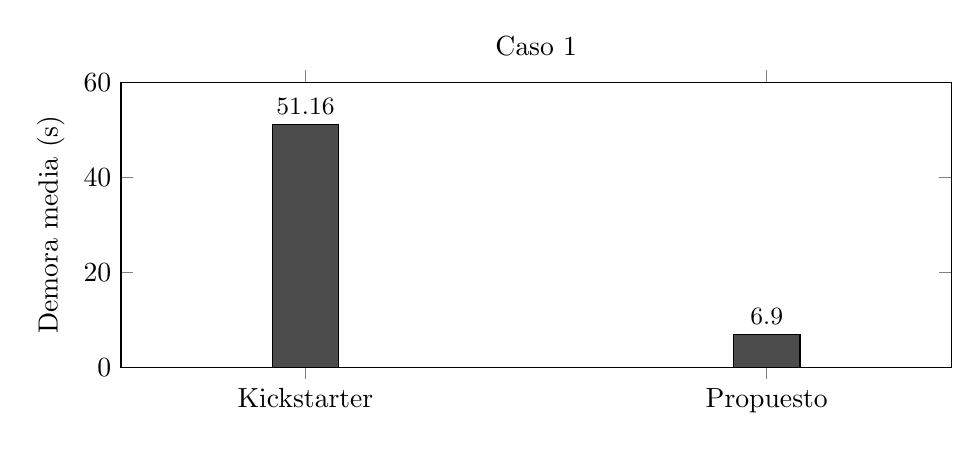
\begin{tikzpicture}
      \begin{axis}[
        width=\linewidth,
        height=5.2cm,
        ybar,
        bar width=24pt,
        ymin=0,
        ymax=60,
        symbolic x coords={Kickstarter,Propuesto},
        xtick=data,
        x tick label style={font=\normalsize},
        ylabel={Demora media (s)},
        title={Caso 1},
        enlarge x limits=0.4,
        nodes near coords,
        nodes near coords align={vertical},
        every node near coord/.append style={font=\small},
      ]
        \addplot[fill=black!70] coordinates {(Kickstarter,51.16) (Propuesto,6.90)};
      \end{axis}
    \end{tikzpicture}
  \end{subfigure}\hfill
  \begin{subfigure}[t]{0.48\textwidth}
    \centering
    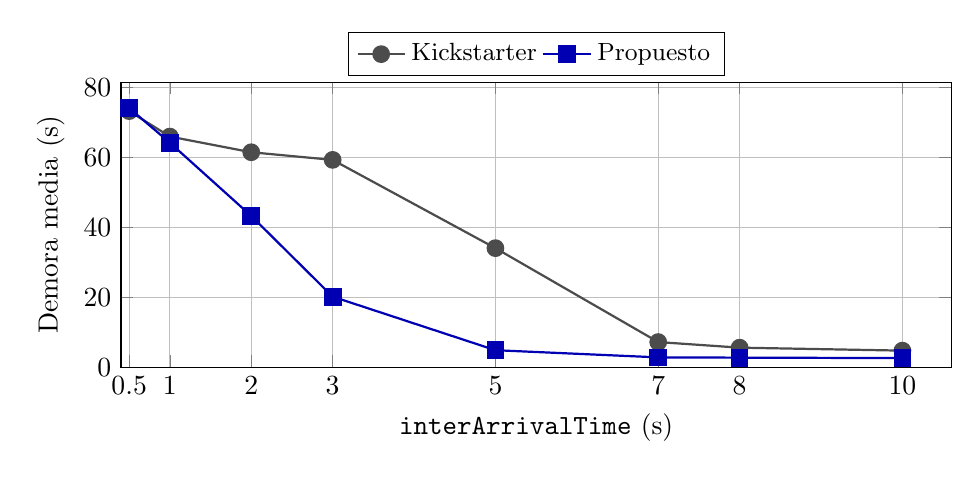
\begin{tikzpicture}
      \begin{axis}[
        width=\linewidth,
        height=5.2cm,
        xmin=0.4, xmax=10.6,
        ymin=0,
        grid=major,
        xlabel={\texttt{interArrivalTime} (s)},
        ylabel={Demora media (s)},
        title={Caso 2},
        xtick={0.5,1,2,3,5,7,8,10},
        legend style={font=\small, at={(0.5,1.02)}, anchor=south, legend columns=-1},
      ]
        \addplot[thick, black!70, mark=*, mark size=2.8pt] coordinates {
          (0.5,73.19) (1,65.92) (2,61.43) (3,59.25) (5,34.01) (7,7.16) (8,5.56) (10,4.71)
        };
        \addplot[thick, blue!70!black, mark=square*, mark size=2.8pt] coordinates {
          (0.5,74.06) (1,64.16) (2,43.22) (3,20.14) (5,4.83) (7,2.78) (8,2.70) (10,2.58)
        };
        \legend{Kickstarter, Propuesto}
      \end{axis}
    \end{tikzpicture}
  \end{subfigure}
  \caption{Comparación de la demora media entre el kickstarter y el algoritmo propuesto. A la izquierda se muestra el Caso~1 y a la derecha el barrido del Caso~2.}
  \label{fig:comparacion-barras}
\end{figure*}

La Fig.~\ref{fig:comparacion-barras} resume la mejora más visible del algoritmo propuesto: en la mayor parte de los escenarios reduce de forma marcada la demora media, con una ganancia especialmente grande cuando la carga ofrecida permite aprovechar ambos sentidos del anillo.

\subsection{Discusión de resultados}

\textbf{\textit{¿Por qué mejoran las métricas?}}

El propuesto elige el camino óptimo en ambas direcciones, ademas el desempate por congestión distribuye tráfico entre ambas direcciones. En enlaces con igual distancia se elige el buffer menos lleno. Es decir tenemos menos saltos, menos demora y al distrubuir la carga, menos espera de buffers.

\begin{figure}[!ht]
  \centering
  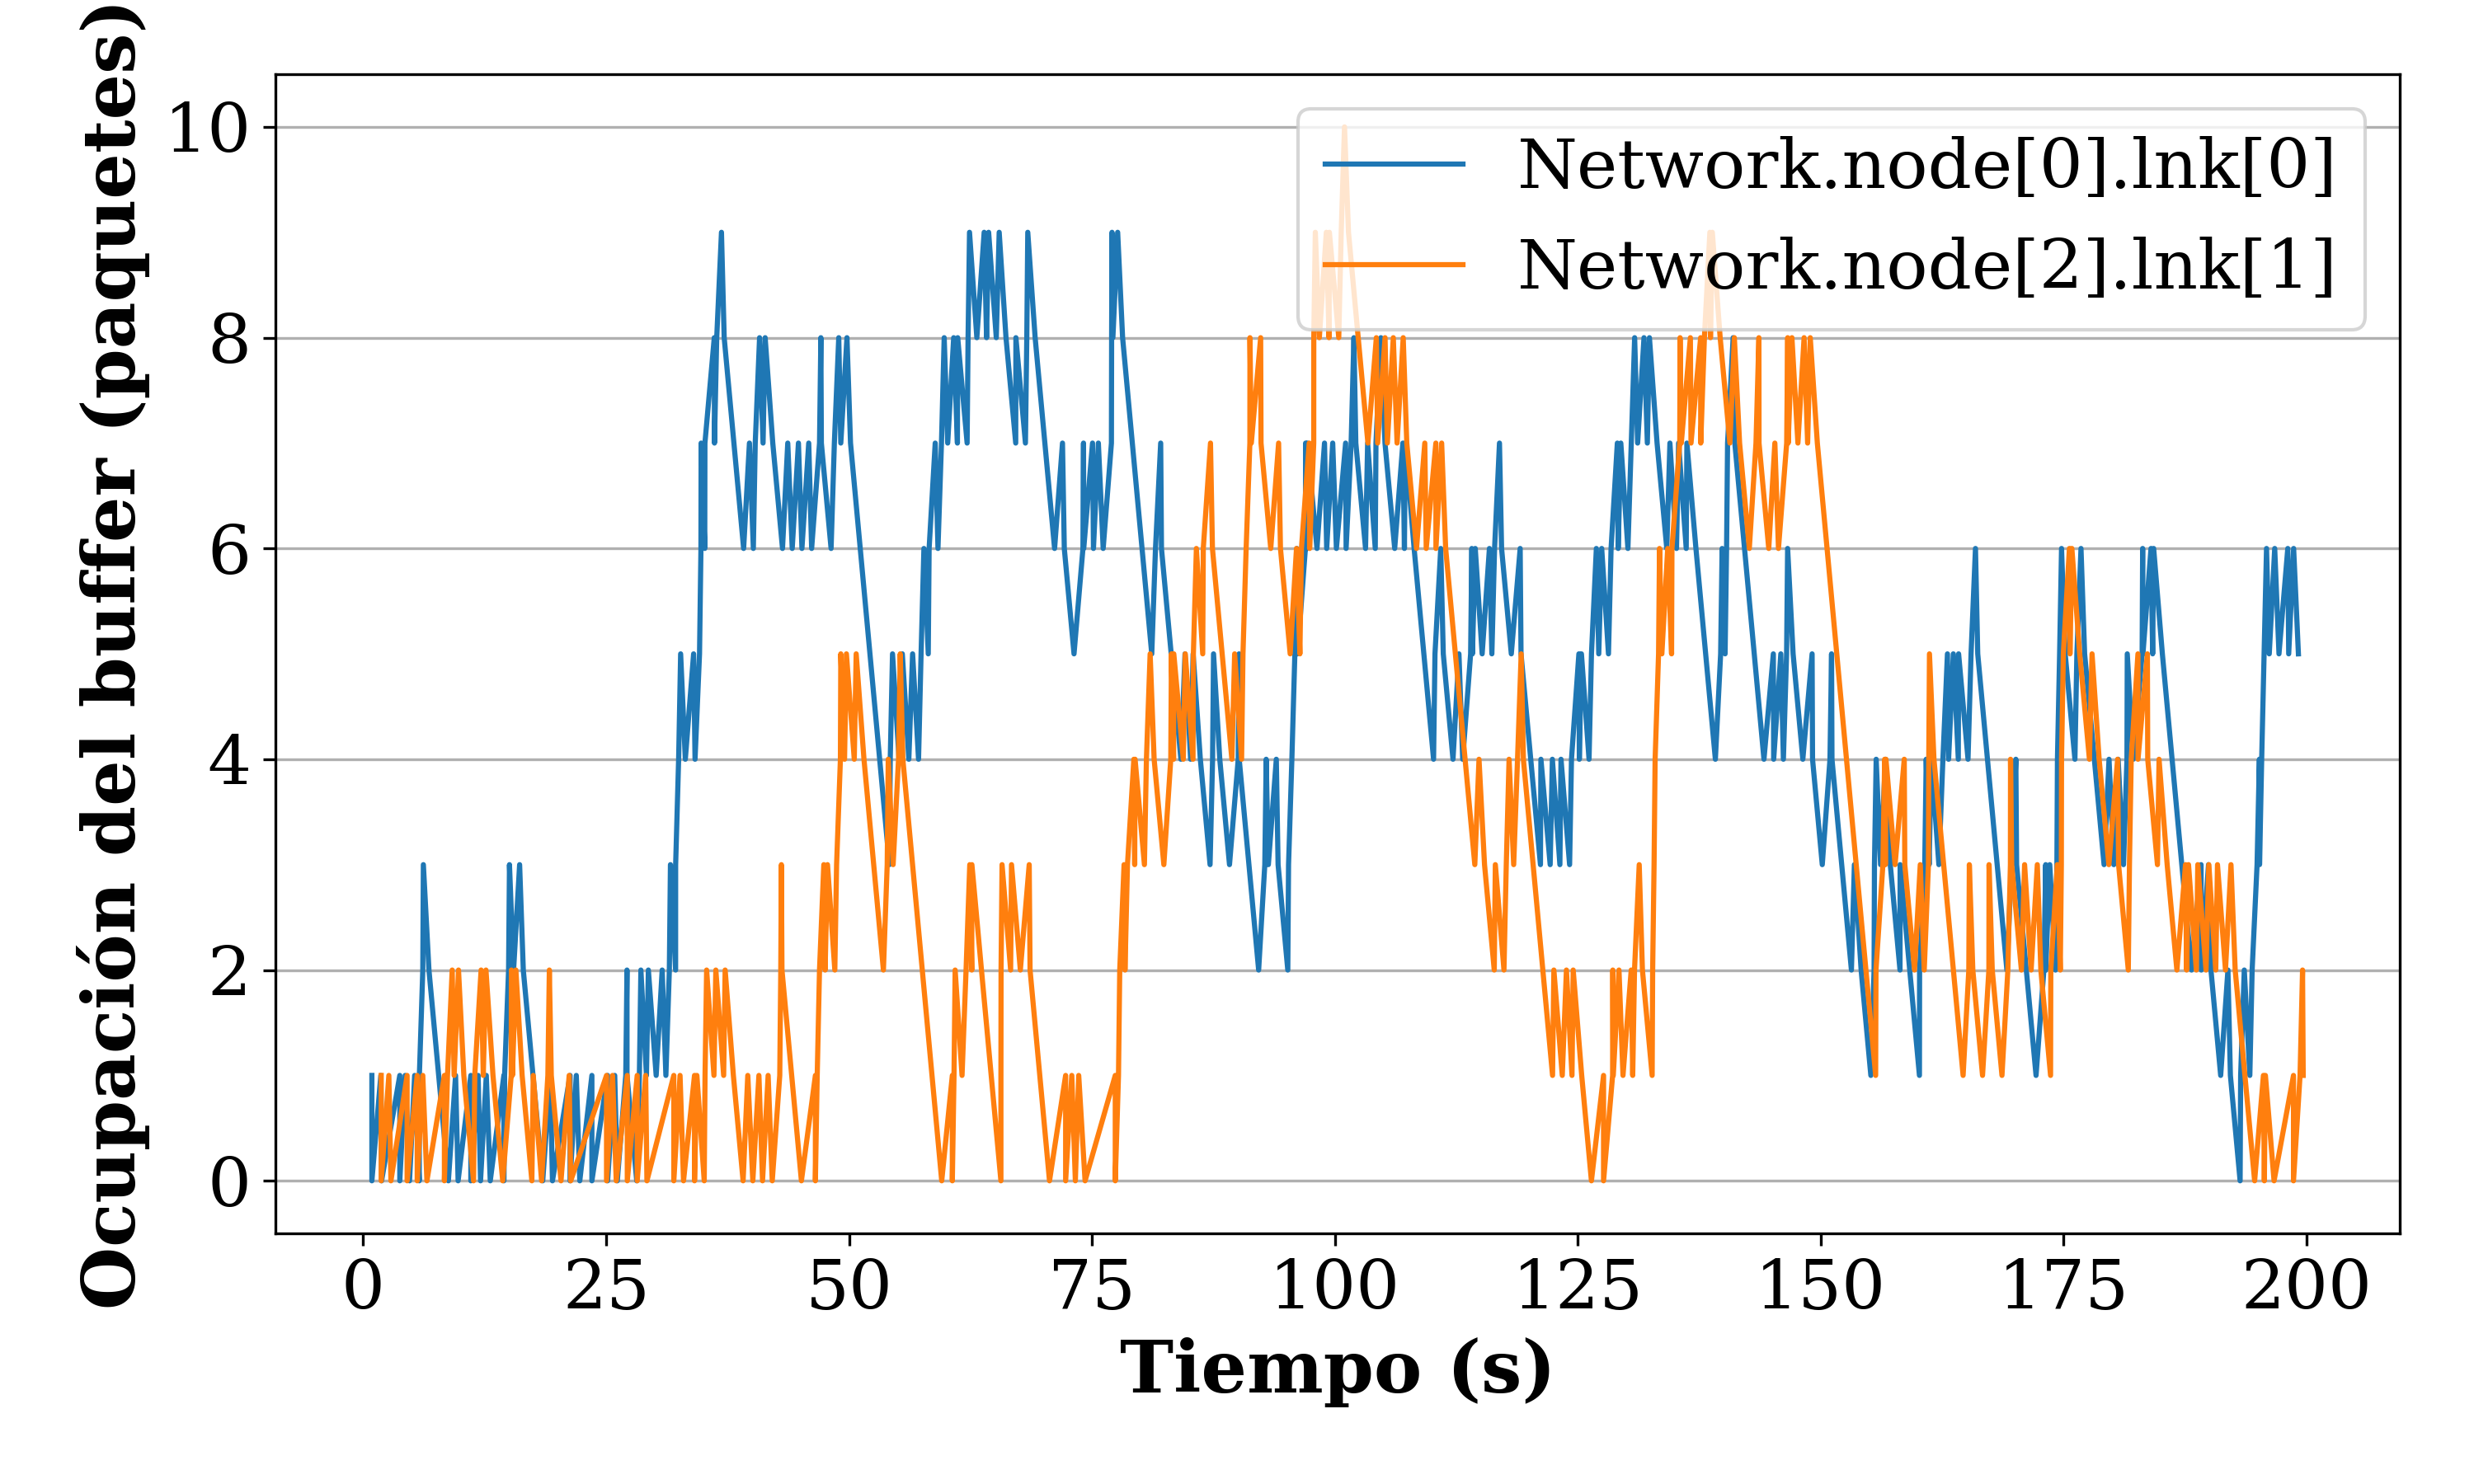
\includegraphics[width=\columnwidth]{../../figuras/entrega-final-caso1_buffers_fuentes.png}
  \caption{Ocupación de buffers a lo largo del tiempo --- nodos fuente, algoritmo propuesto (Caso~1).}
  \label{fig:caso1-propuesto-buffers}
\end{figure}

\begin{figure}[!ht]
  \centering
  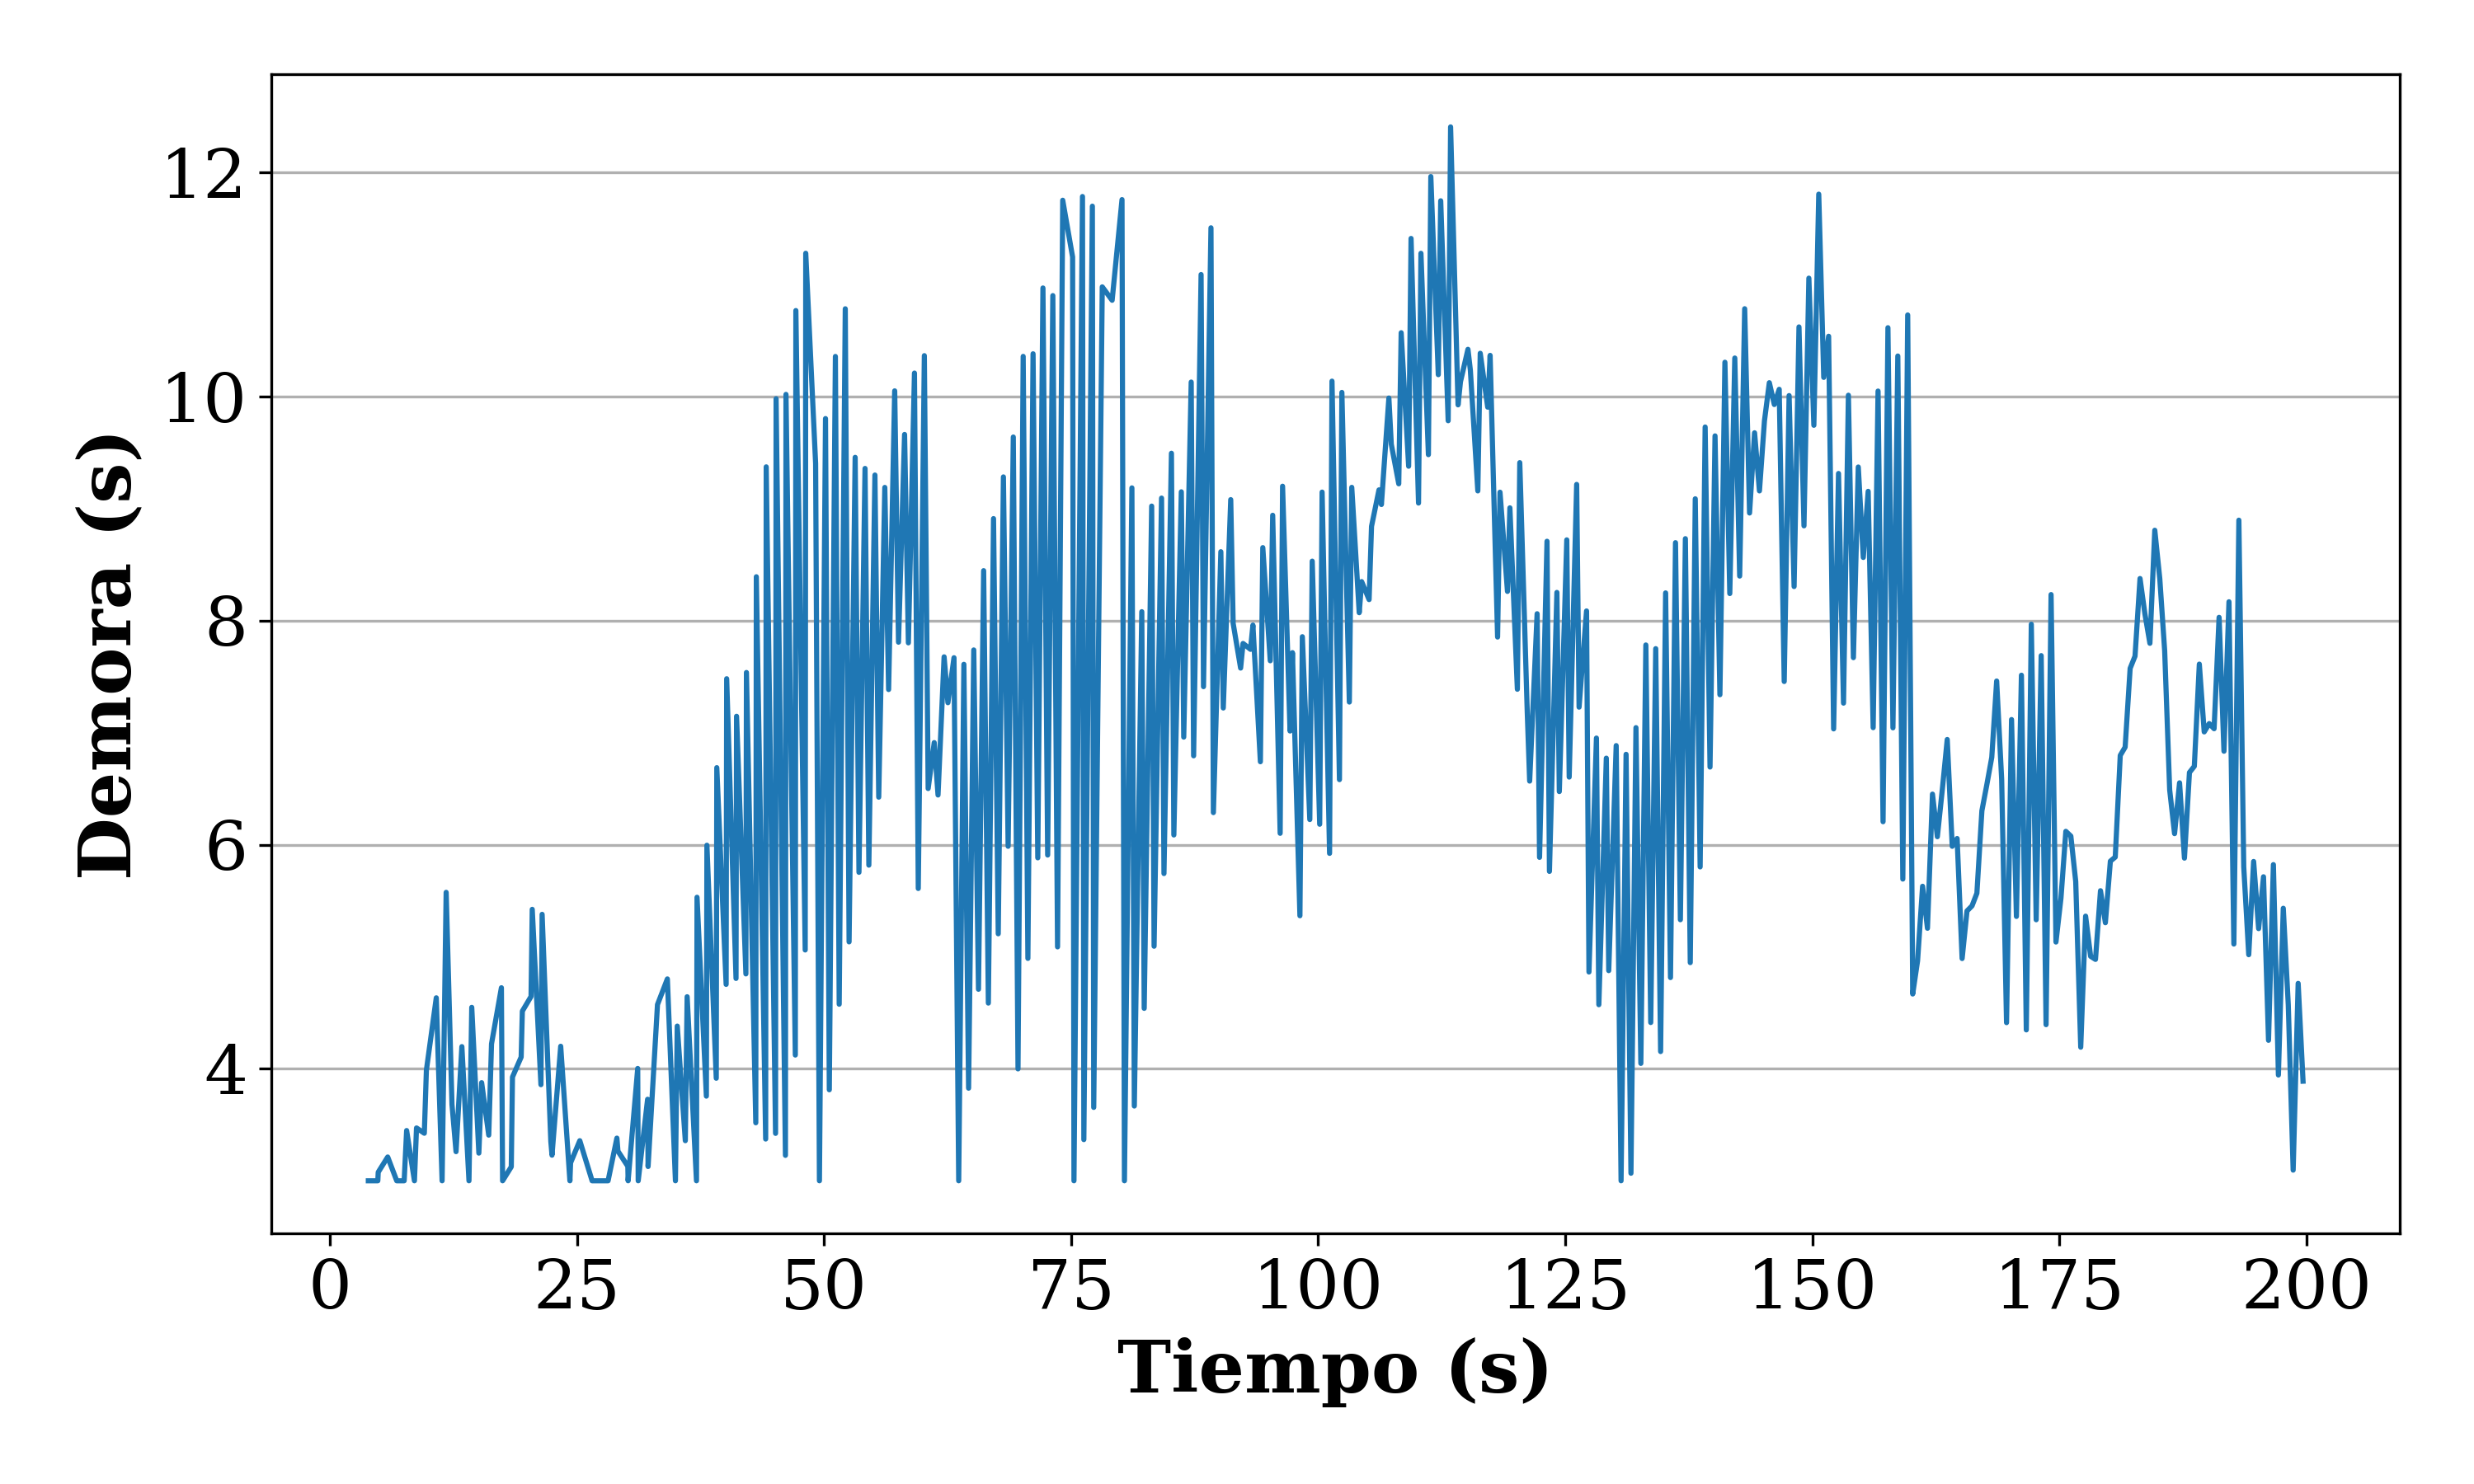
\includegraphics[width=\columnwidth]{../../figuras/entrega-final-caso1_delay.png}
  \caption{Demora extremo a extremo a lo largo del tiempo --- algoritmo propuesto (Caso~1).}
  \label{fig:caso1-propuesto-delay}
\end{figure}

La Fig.~\ref{fig:caso1-propuesto-buffers} muestra la ocupación de buffers de los nodos fuente bajo el algoritmo propuesto. A diferencia del baseline, donde el buffer de \texttt{node[0].lnk[0]} crecía de forma sostenida hasta superar los 190 paquetes, aquí ambos buffers permanecen acotados durante toda la simulación, con un máximo de 10 paquetes. Esto refleja que el uso de ambas direcciones del anillo distribuye la carga y evita la saturación. La Fig.~\ref{fig:caso1-propuesto-delay} confirma este comportamiento: la demora extremo a extremo se mantiene estable y acotada a lo largo de toda la simulación, en contraste con el crecimiento sostenido observado en el baseline.

\FloatBarrier

\textbf{\textit{¿Hubo bucles de enrutamiento?}}

Por la topología de anillo, al solo tener dos direcciones posibles y siempre elegir la más corta nunca nos vamos a encontrar con un bucle. En el peor caso, vamos a recorrer n/2 nodos para llegar al destino.

\textbf{\textit{¿Qué pasaría con muchos más nodos? ¿Cómo escalaría respecto al baseline?}}

El propuesto escala mejor que el baseline porque: Utiliza ambas direcciones (capacidad de red $\times 2$ efectiva) y el calcular las distancias es $O(1)$. Por lo tanto, a medida que el número de nodos crece, la ventaja del propuesto se amplía, reduciendo la demora y evitando saturación en enlaces críticos, mientras que el baseline se vuelve cada vez más ineficiente al concentrar todo el tráfico en un solo sentido del anillo.

\textbf{\textit{¿Qué sucedería si se cae un nodo? ¿Son tolerantes a fallos los algoritmos?}}

El algoritmo propuesto calcula rutas basándose en los indices, y en el caso de que un nodo falle no lo tendríamos en cuenta por lo que ambos son igualmente vulnerables a fallas de nodos críticos.

\FloatBarrier

\section{Conclusiones}
\label{sec:conclusiones}

El kickstarter concentra el tráfico en una sola dirección del anillo y, por eso, satura buffers y aumenta rápidamente la demora cuando la carga crece. En contraste, el algoritmo propuesto aprovecha ambas direcciones, reparte mejor el tráfico y reduce la demora media en la mayoría de los escenarios evaluados, con mejoras muy marcadas en el Caso~1 y en el Caso~2 para cargas medias y bajas.

Además, la decisión basada en distancia y congestión evita bucles y mantiene el costo de decisión en tiempo constante, por lo que la estrategia escala mejor que el baseline cuando la red crece. Como limitación, ambos enfoques siguen siendo vulnerables a fallas de nodos críticos porque no incorporan mecanismos de reconvergencia ni descubrimiento dinámico.

% Bibliografía mínima de ejemplo
\begin{thebibliography}{99}

\bibitem{omnetpp}
A. Varga and R. Hornig, ``OMNeT++,'' in \emph{Proc.\ Int.\ Conf.\ Simulation Tools and Techniques (Simutools)}, 2008.

\bibitem{kickstarter}
Cátedra de Redes y Sistemas Distribuidos, ``Laboratorio 4: kickstarter OMNeT++,'' FaMAF/UNC, 2026.

\bibitem{tanenbaum}
A. S. Tanenbaum and D. J. Wetherall, \emph{Computer Networks}, 5th ed. Upper Saddle River, NJ, USA: Prentice Hall, 2011.

\end{thebibliography}

\end{document}
